%%% DOCUMENTCLASS 
%%%-------------------------------------------------------------------------------

\documentclass[
a4paper, % Stock and paper size.
11pt, % Type size.
% article,
% oneside, 
onecolumn, % Only one column of text on a page.
% openright, % Each chapter will start on a recto page.
% openleft, % Each chapter will start on a verso page.
openany, % A chapter may start on either a recto or verso page.
]{memoir}

%%% PACKAGES 
%%%------------------------------------------------------------------------------
\usepackage{amsthm}
\usepackage[utf8]{inputenc} % If utf8 encoding
% \usepackage[lantin1]{inputenc} % If not utf8 encoding, then this is probably the way to go
\usepackage[T1]{fontenc}    %
\usepackage[english]{babel} % English please
\usepackage[final]{microtype} % Less badboxes
\usepackage{dsfont}
% \usepackage{kpfonts} %Font
\usepackage{amsmath,amssymb,mathtools} % Math

\usepackage{color}
% \usepackage{tikz} % Figures
\usepackage{graphicx} % Include figures

%%% PAGE LAYOUT 
%%%------------------------------------------------------------------------------

\setlrmarginsandblock{0.15\paperwidth}{*}{1} % Left and right margin
\setulmarginsandblock{0.2\paperwidth}{*}{1}  % Upper and lower margin
\checkandfixthelayout

%%% SECTIONAL DIVISIONS
%%%------------------------------------------------------------------------------

\maxsecnumdepth{subsection} % Subsections (and higher) are numbered
\setsecnumdepth{subsection}

\makeatletter %
\makechapterstyle{standard}{
	\setlength{\beforechapskip}{0\baselineskip}
	\setlength{\midchapskip}{1\baselineskip}
	\setlength{\afterchapskip}{8\baselineskip}
	\renewcommand{\chapterheadstart}{\vspace*{\beforechapskip}}
	\renewcommand{\chapnamefont}{\centering\normalfont\Large}
	\renewcommand{\printchaptername}{\chapnamefont \@chapapp}
	\renewcommand{\chapternamenum}{\space}
	\renewcommand{\chapnumfont}{\normalfont\Large}
	\renewcommand{\printchapternum}{\chapnumfont \thechapter}
	\renewcommand{\afterchapternum}{\par\nobreak\vskip \midchapskip}
	\renewcommand{\printchapternonum}{\vspace*{\midchapskip}\vspace*{5mm}}
	\renewcommand{\chaptitlefont}{\centering\bfseries\LARGE}
	\renewcommand{\printchaptertitle}[1]{\chaptitlefont ##1}
	\renewcommand{\afterchaptertitle}{\par\nobreak\vskip \afterchapskip}
}
\makeatother

\chapterstyle{standard}

\setsecheadstyle{\normalfont\large\bfseries}
\setsubsecheadstyle{\normalfont\normalsize\bfseries}
\setparaheadstyle{\normalfont\normalsize\bfseries}
\setparaindent{0pt}\setafterparaskip{0pt}

%%% FLOATS AND CAPTIONS
%%%------------------------------------------------------------------------------

\makeatletter                  % You do not need to write [htpb] all the time
\renewcommand\fps@figure{htbp} %
\renewcommand\fps@table{htbp}  %
\makeatother                   %

\captiondelim{\space } % A space between caption name and text
\captionnamefont{\small\bfseries} % Font of the caption name
\captiontitlefont{\small\normalfont} % Font of the caption text

\changecaptionwidth          % Change the width of the caption
\captionwidth{1\textwidth} %

%%% ABSTRACT
%%%------------------------------------------------------------------------------

\renewcommand{\abstractnamefont}{\normalfont\small\bfseries} % Font of abstract title
\setlength{\absleftindent}{0.1\textwidth} % Width of abstract
\setlength{\absrightindent}{\absleftindent}

%%% HEADER AND FOOTER 
%%%------------------------------------------------------------------------------

\makepagestyle{standard} % Make standard pagestyle

\makeatletter                 % Define standard pagestyle
\makeevenfoot{standard}{}{}{} %
\makeoddfoot{standard}{}{}{}  %
\makeevenhead{standard}{\bfseries\thepage\normalfont\qquad\small\leftmark}{}{}
\makeoddhead{standard}{}{}{\small\rightmark\qquad\bfseries\thepage}
% \makeheadrule{standard}{\textwidth}{\normalrulethickness}
\makeatother                  %

\makeatletter
\makepsmarks{standard}{
	\createmark{chapter}{both}{shownumber}{\@chapapp\ }{ \quad }
	\createmark{section}{right}{shownumber}{}{ \quad }
	\createplainmark{toc}{both}{\contentsname}
	\createplainmark{lof}{both}{\listfigurename}
	\createplainmark{lot}{both}{\listtablename}
	\createplainmark{bib}{both}{\bibname}
	\createplainmark{index}{both}{\indexname}
	\createplainmark{glossary}{both}{\glossaryname}
}
\makeatother                               %

\makepagestyle{chap} % Make new chapter pagestyle

\makeatletter
\makeevenfoot{chap}{}{\small\bfseries\thepage}{} % Define new chapter pagestyle
\makeoddfoot{chap}{}{\small\bfseries\thepage}{}  %
\makeevenhead{chap}{}{}{}   %
\makeoddhead{chap}{}{}{}    %
% \makeheadrule{chap}{\textwidth}{\normalrulethickness}
\makeatother

\nouppercaseheads
\pagestyle{standard}               % Choosing pagestyle and chapter pagestyle
\aliaspagestyle{chapter}{chap} %

%%% NEW COMMANDS
%%%------------------------------------------------------------------------------

\newcommand{\p}{\partial} %Partial
% Or what ever you want
%%% TABLE OF CONTENTS
%%%------------------------------------------------------------------------------

\maxtocdepth{subsection} % Only parts, chapters and sections in the table of contents
\settocdepth{subsection}

\AtEndDocument{\addtocontents{toc}{\par}} % Add a \par to the end of the TOC

%%% INTERNAL HYPERLINKS
%%%-------------------------------------------------------------------------------

\usepackage{hyperref}   % Internal hyperlinks
\hypersetup{
	pdfborder={0 0 0},      % No borders around internal hyperlinks
	pdfauthor={Yannick Couzinié} % author
}
\usepackage{memhfixc}   %

%%% THE DOCUMENT
%%% Where all the important stuff is included!
%%%-------------------------------------------------------------------------------

\author{}
\title{Mathematical Statistical Physics}
\theoremstyle{definition}
\newtheorem{definition}{Definition}[chapter]
\newtheorem{example}[definition]{Example}
\theoremstyle{remark}
\newtheorem{remarks}[definition]{Remarks}
\newtheorem{notes}[definition]{Notes}
\theoremstyle{plain}
\newtheorem{theorem}[definition]{Theorem}
\newtheorem{prop}[definition]{Proposition}
\newtheorem{lemma}[definition]{Lemma}
\begin{document}
\setlength{\parindent}{0pt}
\maketitle
\tableofcontents

\newpage\chapter{Preliminary stuff}
In the Heisenberg picture of quantum mechanics there are three core principles: \begin{enumerate}
	\item Central objects are the observables, which are realized as operators on a Hilbert space.
	\item Time evolution acts on observables.
	\item Auxiliary objects are the states, realized as vectors on the Hilbert space, used to compute expectation values of observables.
\end{enumerate}
This is a notion heavily based on physical intuition. One can translate these three principles into a mathematical formulation in the following way: \begin{enumerate}
	\item The set of observables is a \textit{C*-algebra} $\mathcal{A}$, namely: \begin{itemize}
		\item $\mathcal{A}$ is an associative algebra.
		\item $\mathcal{A}$ is equipped with a norm such that $\|A\cdot B\| \leq \| A \|\cdot \| B\| $.
		\item It is complete with respect to $\| \cdot \|$.
		\item It is equipped with an involution $*:\mathcal{A}\rightarrow \mathcal{A}$ such that \begin{align}
		(A^*)^*&=A\\
		(A+\lambda B)^* &= A^* +\overline{\lambda}B^*\\
		(AB)^*&=B^*A^*
		\end{align}
		\item $C^*$-property, i.e. $\|A^*A\|=\|A\|^2$.
	\end{itemize}
\begin{remarks}
	There is a lot to be said about $C^*$-algebras but we will keep it short. \begin{enumerate}
		\item Observables $A\in\mathcal{A}$ are not required to be self-adjoint ($A=A^*$).
		\item In the quantum mechanic setting $\mathcal{H}$ is a Hilbert space, then one takes the ''set of bounded operators'' $\mathcal{A}=\mathcal{L}(\mathcal{H})$.
		\item Physically, there are unbounded observables. At least for self-adjoint ones $A=A'$, one can consider equivalently the unitary correspondents $U=e^{itA}$, since there is a one-to-one correspondence by Stokes' theorem.
		\item $\mathcal{A}$ does not need to have a $\mathds{1}$.
	\end{enumerate}
\end{remarks}
\item A pair $(\mathcal{A},\tau)$ is a $C^*$-dynamical system if $\mathcal{A}$ is a $C^*$-algebra and $\mathbb{R}\ni t\mapsto \tau_t$ is a strongly continuous one-parameter group $*-$automorphism of $\mathcal{A}$: \begin{itemize}
	\item $\tau_t:\mathcal{A}\rightarrow \mathcal{A}$ such that \begin{align}
	\tau_t(A^*)&=(\tau_t(A))^*\\
	\tau_t(A+\lambda B)&=\tau_t(A)+\lambda\tau_t(B)\\
	\tau_t(AB)&=\tau_t(A)\tau_t(B)\\
	\|\tau_t(A)\|&=\|A\|\; .
	\end{align}
	\item $\tau_0(A)=A; \tau_{t+s}=\tau_t(\tau_s(A))$ \; .
	\item For any $A\in \mathcal{A}$, $\| \tau_{t+\varepsilon}(A)-\tau_{t}(A)\|\rightarrow 0 (\varepsilon \rightarrow 0)$, i.e. uniformity in $A$.
\end{itemize}
\begin{remarks}
	$\tau$ is always generated by a $*$-derivation of the form \begin{align}
	\delta_t:\mathcal{A}&\longrightarrow \mathcal{A}\\
	A&\longmapsto t^{-1}(\tau_t(A)-A)\; .
	\end{align}
	The domain is defined as $D(\delta)=\{A\in\mathcal{A} \mid \lim\limits_{t\rightarrow 0}\delta_t(A) \text{ exists}\}$ for which we then have \begin{align}
	\delta: D(\delta)&\longrightarrow \mathcal{A}\\
	A&\longmapsto \delta(A)=\lim_{t\rightarrow 0}\delta_t(A)\; .
	\end{align}
	Then $\delta$ is a closed, densely defined map such that \begin{align*}
	\mathds{1}\ni D(\delta), \delta(\mathds{1})&=0\\
							\delta(AB)&=\delta(A)B+A\delta(B)\\
							\delta(A^*)&=\delta(A)^*\;  .
	\end{align*}
	In fact, there is a one-to-one correspondence between $\tau_t$ and $\delta$ (Hille-Yoshida).
\end{remarks}
\begin{remarks}
	In the quantum mechanic setting $\mathcal{A}=\mathcal{L}(\mathcal{H})$. The dynamics are generated by a $H\cdot H^*$ on $\mathcal{H}$, namely \begin{align}
	\tau_t(A)=e^{itH}Ae^{-itH}\; .
	\end{align}
	It is a $*$-automorphism by unitarity of $e^{-itH}$ and a strongly continuous group because $t\mapsto e^{-itH}$ is so. The $*$-derivation is given by \begin{align*}
	\delta(A)=\frac{\mathrm{d}}{\mathrm{d}t}\tau_t(A)\mid_{t=0}=i[H,A]\; ,
	\end{align*}
	sometimes written as $\tau_t(A)=e^{i[H,\cdot]t}(A)$.
\end{remarks}
\item Finally, a \underline{state} over $A$ is a positive, normalized linear functional over $A$ \begin{align*}
\omega:\mathcal{A}&\longmapsto \mathbb{C}\\
A&\longrightarrow \omega(A)\in\mathbb{C}\; ,
\end{align*}
such that $\omega(A^*A)\geq 0$ (positivity) and $\|\omega \| :=\sup \frac{\|\omega(A)\|}{\|A\|}=1$ (normalization).
\begin{remarks}
	Let us now try to establish some intuition \begin{itemize}
		\item The positivity of the quadratic function $\lambda\mapsto \omega((A+\lambda B)^*(A+\lambda B))$ implies 
		\begin{enumerate}
			\item $\omega(A^*B)=\omega(B^*A)$.
			\item $|\omega(A^*B)|^2\leq \omega(A^*A)\omega(B^*B)$ (Cauchy-Schwarz inequality).
		\end{enumerate}
		\item In the quantum mechanic setting, any normalized vector $\psi\in\mathcal{H}$ defines a state by \begin{align}\omega_{\psi}:\mathcal{A}&\longrightarrow \mathbb{C}\\
		A&\longmapsto \langle \psi, A\psi\rangle \; .\end{align}
		\item Also any density matrix $\varrho = \varrho^*\in \mathcal{L}(\mathcal{H})$ defines a state by \begin{align}
		\omega_{\varrho}:A&\longrightarrow \mathbb{C}\\
		A&\longmapsto \omega_{\rho}(A)=\mathrm{Tr}(\varrho A) \qquad (\mathrm{Tr}(\varrho)=1) \; .
		\end{align}
		\item If $\mathds{1}\in\mathcal{A}$, then $\omega$ is normalized $\Leftrightarrow$ $\omega(\mathds{1})=1$.
		\end{itemize}
\end{remarks}
\end{enumerate}
It turns out that $\mathcal{A}$ may have inequivalent representations, corresponding to thermodynamically different situations. A representation of the $C^*$-algebra $A$ on a Hilbert-space $\mathcal{H}$ is a $*$-morphisms
$\pi:\mathcal{A}\longrightarrow \mathcal{L}(\mathcal{H})$, namely \begin{align}
\pi(A\cdot B)&=\pi(A)\pi(B) \\
\pi(A+\lambda B)&=\pi(A)+\lambda\pi(B)\\
\pi(A^*)&=(\pi(A))^*\;.
\end{align}
$\pi_1,\pi_2$ are called equivalent if there is a unitary map \begin{align}
U:\mathcal{H}_1\rightarrow \mathcal{H}_2 \text{ s.t. } U\pi_1(A)=\pi_2(A)U\quad \forall A\in \mathcal{A}\; .
\end{align}
Now given a $\pi$ on $\mathcal{H}$ and any normalized vector $\xi\in\mathcal{H}$, then the map \begin{align}
\omega_{\xi}:\mathcal{A}&\longrightarrow \mathbb{C}\qquad \omega_{\xi}(A)=\langle\xi,\pi(A)\xi\rangle \; ,
\end{align}
defines a state on the algebra. Given a state $\omega$ on $\mathcal{A}$, there exists a $\mathcal{H}_{\omega}$, a representation $\pi_{\omega}:\mathcal{A}\rightarrow \mathcal{H}_{\omega}$ and a normalized $\Omega_{\omega}\in\mathcal{H}_ra{\omega}$ such that \begin{align}
\omega(A)=\langle\Omega_{\omega},\pi_{\omega}(A)\Omega_{\omega}\rangle \quad \text{''GNS construction''.}
\end{align}
We will be mainly using two topologies \begin{enumerate}
	\item In $\mathcal{A}$: $A_n\rightarrow A$ if $\|A_n-A\|\rightarrow 0$. 
	\item In a representation where $\mathcal{A}$ is represented as $\mathcal{L}(\mathcal{H})$ there: uniform convergence, strong convergence, weak convergence apply as usual, outside of representations, these terms do not make sense.
\end{enumerate}
\begin{remarks}
	On the set of states over $\mathcal{A}$, designated by $\varepsilon(\mathcal{A})$, one has \begin{itemize}
		\item $\varepsilon(\mathcal{A})$ is a convex set. $\omega_1,\omega_2\in\varepsilon(\mathcal{A})$ then $\omega=\lambda\omega_1+\mu\omega_2\in\varepsilon(\mathcal{A})$.
		\item $\varepsilon(\mathcal{A})$ is weakly-$*$ compact (if $\mathcal{A}$ has an identity), namely every sequence $(\omega_n)_{n\in\mathcal{N}}$ of states in $\mathcal{A}$ has convergent subsequences (in the weak-$*$-topology) $\exists(n_k)_{k\in\mathcal{N}}:\omega_{n_k}(A)\rightarrow \overline{\omega}(A)$.
	\end{itemize}
In particular: A sequence of finite volume thermal equilibrium states always have infinite-volume limit points. As we shall see later, the uniqueness of the infinity point can be takes as a characterization of phase transitions.
\end{remarks}
\chapter{Ideal gases}
The ideal gas is a gas of non-interacting particles. The thermodynamic limit (TDL) is usually obtained by taking $N$ particles in a  finite volume $\Lambda\in \mathbb{R}^d$ and letting $N\rightarrow\infty$, $\Lambda\rightarrow\mathbb{R}^d$ such that \begin{align}
N/|\Lambda|\rightarrow \varrho \qquad \text{ with } \qquad 0<\varrho < \infty.
\end{align}
There are two types of indistinguishable particles in nature \begin{enumerate}
	\item Bosons have a symmetric wave function.
	\item Fermions have an antisymmetric wavefunction.
\end{enumerate}
A Hilbert space carrying an arbitrary number of particles is a Fock space built upon the one-particle Hilbert space. Action of the symmetric group $S_n$ on $\otimes^N\mathcal{H}$ is then given by \begin{align}
P_{\sigma}:\psi_1\otimes \cdots \otimes \psi_N \longmapsto {\psi}_{\sigma^{-1}(1)}\otimes \cdots \otimes \psi_{\sigma^{-1}(N)}\; ,
\end{align}
for any $\sigma\in S_n$ (check $P_{\sigma\sigma'}=P_{\sigma}\circ P_{\sigma'}$ and so on) and one defines the space of (anti-)symmetric wavefunctions as \begin{align}
\mathcal{H}_{s/a}^{N}&:=\{\psi\in\otimes^N\mathcal{H}:P_{\sigma}\psi=\delta(\sigma)\psi \text{ for any } \sigma\in S_n\}\; ,\\\delta(\sigma)&=\begin{cases}
1 &\text{ if ''s'' (Bosons)}\\
-1 &\text{ if ''a'' (Fermions)}
\end{cases}\; .
\end{align}
Furthermore one has $\mathcal{H}_{s/a}^0:=\mathbb{C}$ with unit vector $\Omega$, called ''vacuum''. Now the Fock space is given by \begin{align}
\mathcal{F}_{s/a}(\mathcal{H})=\bigoplus_{N\in\mathbb{N}\cup\{0\}}\mathcal{H}_{s/a}^N\; ,
\end{align}
$\psi\in\mathcal{F}_{s/a}(\mathcal{H})$ is represented as $(\psi^N)_{N\in\mathbb{N}\cup\{0\}}=(\psi^0,\psi^1,\ldots)$ where $\psi^N\in\mathcal{H}^N_{s/a}$ with the norm given by \begin{align}
\|\psi\|^2_{\mathcal{F}_{s/a}(\mathcal{H})}=\sum_{N\geq 0}\|\psi^N\|^2_{\otimes^N\mathcal{H}}\; .
\end{align}
\begin{remarks}
	\begin{itemize}
		\item This sum has to be convergent, thus the series elements have to decrease in value. Since the probability to have more than $M$ particles is given by taking the sum $\sum_{N\geq M}\|\psi^N\|^2_{\otimes^N\mathcal{H}}$ one can conclude that the Fock space does not describe the infinite particle state as for $M\rightarrow\infty$ the state would always be zero. One can only take the TDL.
		\item The number operator is given by $(\mathcal{N}\psi)^N=N\psi^N$ for any $N\in \mathbb{N}$.
		\item Second quantization: If $A:\mathcal{H}\rightarrow \mathcal{H}$ is a linear operator then define $\Gamma(A),\mathrm{d}\Gamma(A):\mathcal{H}_{s/a}^N\rightarrow \mathcal{H}_{s/a}^N$ for any $N$ where \begin{align}
		\Gamma(A)&=A\otimes \cdots \otimes A\\
		\mathrm{d}\Gamma(A)&=\sum_{j=1}^N\mathds{1}\otimes\cdots\otimes \mathds{1}\otimes \underbrace{A}_{\text{j-th position}}\otimes \mathds{1}\cdots \otimes \mathds{1}\;,
		\end{align}
		with which one has $N=\mathrm{d}\Gamma(\mathds{1})$. Also if $A$ is self-adjoint then $\frac{\mathrm{d}}{\mathrm{d}t}\Gamma(e^{itA})\mid_{t=0}=i\mathrm{d}\Gamma(A)$ i.e. $\Gamma(e^{itA})=e^{itd\Gamma(A)}$.
	\end{itemize}
\end{remarks}
The core concepts of Fock spaces are those of annihilation and creation operators: \begin{itemize}
	\item Annihilation operators: For $\varphi\in\mathcal{H}$ one defines \begin{align}
	b(\varphi):\otimes^N\mathcal{H}&\longrightarrow \otimes^{N-1}\mathcal{H}\\
	b(\varphi)(\psi_1\otimes\ldots\otimes\psi_N)&=\sqrt{N}\langle \varphi,\psi_1\rangle_{\mathcal{H}}~\psi_2\otimes\ldots\otimes\psi_N\\
	b(\varphi)\Omega &= 0\; .
	\end{align}
	Since $b(\varphi):\mathcal{H}_{s/a}^N\rightarrow \mathcal{H}_{s/a}^{N-1}$ for any $N$, it extends to a map $b(\varphi):\mathcal{F}_{s/a}(\mathcal{H})\rightarrow \mathcal{F}_{s/a}(\mathcal{H})$.
	\item Creation operators: For $\varphi\in\mathcal{H}$ one defines \begin{align}
	b^*(\varphi)\psi^{N-1}&=\frac{1}{\sqrt{N}}\sum_{k=1}^{N}(\pm 1)^{k-1}P_{\pi_k}(\varphi\otimes \psi^{N-1}) \text{ where $\pm$ is for $s/a$ and}\\
	\pi_k^{-1}&=(k,1,2,\cdots,k-1,k+1,\cdots,N)\; .
	\end{align}
	This can be interpreted as inserting a particle $\varphi$ into each position and average over the possible positions, that's what $P_{\pi_k}$ does, inserting into the $k$-th position. Proving this exactly is cumbersome.
	\end{itemize}
\begin{remarks}
	\begin{itemize}
		\item $b^*(\varphi)=(b(\varphi))^*$.
		\item $\varphi\mapsto b(\varphi)$ is anti-linear, i.e. $\varphi\mapsto b^*(\varphi)$ is linear.
		\item The following commutation law holds $Nb(\varphi)=b(\varphi)(N-1)$. 
		\item If $U:\mathcal{H}\rightarrow\mathcal{H}$ is unitary: $\Gamma(U)b^*(\varphi)\Gamma(U)^*=b^*(U\varphi)$.
		\item The following commutation relations hold on $\mathcal{F}_s(\mathcal{H})$ (CCR) \begin{align}
		[b(\varphi),b^*(\psi)]&=\langle\varphi,\psi\rangle\mathds{1}\\
		[b(\varphi),b(\psi)]&=[b^*(\varphi),b^*(\psi)]=0\; .
		\end{align}
		\item Canonical anticommutation relation on $\mathcal{F}_a(\mathcal{H})$ (CAR)\begin{align}
		\{b(\varphi),b^{\dagger}(\psi)\}&=\langle\varphi,\psi\rangle \mathds{1}\\
		\{b(\varphi),b(\psi)\}&=\{b^*(\varphi),b^*(\psi)\}=0\; ,
		\end{align}
		where $\{A,B\}=AB+BA$.
	\end{itemize}
\end{remarks}
\section{Fermions}
The (CAR) relations indicate that the fermionic creation/anihilation operators are a representation of the abstract algebra $CAR(\mathcal{H})$, defined as the $C^*$-algebra generated by $\mathds{1}$ and $a(\varphi), \varphi\in\mathcal{H}$ satisfying: \begin{align}
	&\varphi\mapsto a(\varphi) \text{is antilinear}\; ,\\
	&\{a(\varphi),a(\psi)^*\}=\langle\varphi,\psi\rangle \label{eqn::comm_car}\\
	&\{a(\varphi), a(\psi)\} =0=\{a(\varphi)^*,a(\psi)^*\}. 
\end{align}
Since \begin{align}
(a(\varphi)^*a(\varphi))^2=&a(\varphi)^*\{a(\varphi),a(\varphi)^*\}a(\varphi)\\
=&\|\varphi\|^2a(\varphi)^*a(\varphi)\;,\end{align}
so by taking the norm on both sides and applying the $C^*$-property one finds \begin{align}
&\|a(\varphi)^*a(\varphi)\|^2=\|\varphi\|^2\|a(\varphi)^*a(\varphi)\|\\
\Rightarrow&\|a(\varphi)^*\|=\|\varphi\|\; ,
\end{align}
i.e. that the map $\varphi\mapsto a(\varphi)^*$ is continuous. \begin{remarks}
	\begin{itemize}
		\item If $h$ is a pre-Hilbert space, with $\overline{h}=\mathcal{H}$, then $CAR(h)=CAR(\mathcal{H})$.
		\item $CAR(\mathcal{H})$ is unique up to $*$-isomorphisms.
	\end{itemize}
\end{remarks}
\begin{example} Consider Thermal equilibrium in a finite volume $\Lambda \subset C\mathbb{R}^d$. The \textit{Gibbs state} at inverse temperature $0<\beta<\infty$ and chemical potential $\mu\in\mathbb{R}$ is given by \begin{align}
w_{\beta,\mu}^{\Lambda}(A):=Z^{-1}_{\beta,\mu} \mathrm{Tr}(e^{-\beta K_{\mu}}A)\; ,\label{Eqn::def_gibbs_state}
\end{align}
where $A\in \mathrm{CAR}(\mathcal{H}_1)$ and $K_{\mu}=\mathrm{d}\Gamma(H-\mu\mathds{1})=\mathrm{d}\Gamma(H)-\mu\mathcal{N}$ and \begin{align}
Z_{\beta,\mu}=\mathrm{Tr}(e^{-\beta K_{\mu}})\; ,
\end{align}
whenever $\exp(-\beta K_{\mu})\in I_1(\mathcal{F}_a(\mathcal{H}_1))$ (trace-class operator).\end{example}
\begin{lemma}
	$\exp(-\beta H)\in I_1(\mathcal{H}_1)\Leftrightarrow \exp(-\beta K_{\mu})\in I_1(\mathcal{F}_a(\mathcal{H}_q))\forall\mu\in \mathbb{R}$.
\end{lemma}
\begin{example}
	$\Lambda=[-L/2,L/2], \mathcal{H}_1=L^2(\Lambda), H=-\Delta_L$.

\underline{But} $-\Delta$ on $\mathbb{R}^d$ has purely absolutely continuous spectrum so $\exp(\Delta)$ cannot be trace-class. Defining the activity Z as \begin{align}
z=e^{\beta\mu}\; ,
\end{align}
one can find the following relation \begin{align}
\exp(-\beta K_{\mu})&=\Gamma(\exp(-\beta(H-\mu\mathds{1})))=z\Gamma(\exp(-\beta H))\\
e^{-\beta K_{\mu}}b^{\#}(\varphi)&=zb^{\#}(e^{-\beta H}\varphi)e^{-\beta K_{\mu}}\label{eqn::hashtag_eqn}\; ,
\end{align}
whereby the hashtag is a placeholder for nothing or dagger.
\begin{prop}
	If $\exp(-\beta H)\in I_1(\mathcal{H}_1)$, then the Gibbs states are given by\begin{align}
	\omega_{\beta,\mu}(a^{*}(\varphi)a(\psi))&=\langle \psi, ze^{-\beta H}(1+ze^{-\beta H})^{-1}\varphi\rangle\\
	\omega_{\beta,\mu}(a^*(\varphi))&=0=\omega_{\beta,\mu}(a(\varphi))\; .
	\end{align}
\end{prop}
\begin{proof}
	The proof uses first the definition of Gibbs state in Eq. \eqref{Eqn::def_gibbs_state} and then Eq. \eqref{eqn::hashtag_eqn} giving in the first line\begin{align}
	\omega_{\beta,\mu}(a^{*}(\varphi)a(\psi))=~~&Z^{-1}_{\beta,\mu}\mathrm{Tr}(zb^*(e^{-\beta H}\varphi)e^{-\beta K_{\mu}}b(\psi)) \mid \text{cycl. of tr}\\
	=~~&z\omega_{\beta,\mu}(a(\psi)a^*(e^{-\beta H}\varphi)) \\
	\overset{\eqref{eqn::comm_car}}{=}& -z\omega_{\beta,\mu}(a^*(e^{-\beta H}\varphi)a(\psi))\langle \psi, ze^{-\beta H}\varphi\rangle\\
	=~~&-\omega_{\beta,\mu}(a^*(ze^{-\beta H}\varphi)a(\psi))\langle \psi, ze^{-\beta H}\varphi\rangle\\
	\Rightarrow \omega_{\beta,\mu}(a^*((\mathds{1}+ze^{-\beta H})\varphi)a(\psi))=~~&\langle \psi, ze^{-\beta H} \varphi\rangle\; .
	\end{align}
Since $ze^{-\beta H}>0$ implies that $(\mathds{1}+ze^{-\beta H})$ is invertible, this yields the first part of the claim.\\
	If $\psi$ is such that $\mathcal{N}\psi= N\psi$ (i.e. fixed particle number) then \begin{align}
	\langle \psi,e^{-\beta K_{\mu}}b(\varphi)\psi\rangle &={N}^{-1}\langle \psi , e^{-\beta K_{\mu}}(\mathcal{N}+1)b(\varphi)\psi\rangle\\
	&= N^{-1}\langle \psi, (\mathcal{N}+1)e^{-\beta K_{\mu}}b(\varphi)\psi\rangle\\
	&=\frac{N+1}{N}\langle \psi, e^{-\beta K_{\mu}}b(\varphi)\psi\rangle\\
	\Rightarrow \langle \psi,e^{-\beta K_{\mu}}b(\varphi)\psi\rangle&=0\; .
	\end{align}
	Computing $\mathrm{Tr}(e^{-\beta K_{\mu}}b(\varphi))$ in a basis of such vectors proves the claim. Now: By a similar argument \begin{align}
	\omega_{\beta,\mu}(a^*(\varphi_1)\cdots a^{*}(\varphi_n)a(\psi_m)\cdots a(\psi_1))=\delta_{n,m}\det\left(\{\langle\psi_i,\varrho\varphi_j\rangle\}_{i,j=1}^{n}\right)\; ,	\end{align}
$\text{where }\varrho = ze^{-\beta H}(\mathds{1}+ze^{-\beta H})^{-1}$.
\end{proof}
\end{example}
\begin{remarks}
	The \textit{2n-point function} is expressed in terms of the 2-point function $\langle \psi, ze^{-\beta H}(\mathds{1}+ze^{-\beta H})^{-1}\varphi\rangle$ called \textit{Gaussian state} or \textit{quasi-free state}.
\end{remarks}
\begin{remarks}
	The crucial property used in this calculation, expressed in Eq. \eqref{eqn::hashtag_eqn}, is the so called \textit{KMS condition} (which is adressed in further detail in Sec. \ref{sec::kms_states}) \begin{align}
	\omega_{\beta,\mu}(BA)&=\omega_{\beta,\mu}(A\tau_{i\beta}(B))\\
	&=\omega_{\beta,\mu}(Ae^{\beta K_{\mu}}Be^{-\beta K_{\mu}})\; .
	\end{align}
\end{remarks}
The next question is how one takes the TDL, which means here that $\mathcal{H}\rightarrow L^2(\mathbb{R}^d)$, then one has to take the limit of the operators \begin{align}
(H\psi)(x)=(-\Delta \psi)(x)=(2\pi)^{-d/2}\int |\xi|^2\hat{\psi}(\xi)e^{i\xi\cdot x}\mathrm{d}\xi\; .
\end{align}
How can one evaluate this? The dynamics on $CAR(\mathcal{H})$ are given by $\tau_t(a^{\#}(\varphi))=a^{\#}(e^{-itH}\varphi)$. As per usual, one takes the well understood finite case $f(-\Delta_L)$ which converges to $f(-\Delta)$ strongly for any bounded, continuous function f. This applies to $e^{-itx}$, $e^{-\beta x}$, $ze^{-\beta x}(1+ze^{-\beta x})^{-1} (\text{for }x>0)$.
\begin{theorem}
	Let $\omega_{\beta,\mu}^L$ be the Gibbs state associated to $H_L=-\Delta_L$ on $CAR(\mathcal{H}_L)$. Then \begin{align*}
	\omega_{\beta,\mu}^L(A)\overset{}{\longrightarrow}\omega_{\beta,\mu}(A) \qquad (L\rightarrow \infty)\; ,
	\end{align*}
	for any $A\in CAR(\mathcal{H}_{L})$ and any $L$, where $\omega_{\beta,\mu}$ is the quasi-free state over $CAR(\mathcal{H})$ with the two-point function \begin{align}
		\omega_{\beta,\mu}(a^*(\varphi)a(\psi))=(2\pi)^{-d/2}\int\overline{\hat{\psi}(\xi)}\frac{ze^{-\beta |\xi|^2}}{1+ze^{-\beta|\xi|^2}}\hat{\varphi}(\xi)\mathrm{d}\xi\; .
	\end{align}
\end{theorem}
\begin{proof}
We can limit ourselves to $\varphi,\psi\in C_c^{\infty}(\mathbb{R}^d)$, since $\mathrm{CAR}(C_C^{\infty})$ is equal to $\mathrm{CAR}(L^2(\mathbb{R}^d))$ as $C_c^{\infty}(\mathbb{R^d})$ is dense in $L^2(\mathbb{R}^d)$.
	It suffices to prove the statement for the two-point function, due to the above Proposition. But this follows from the weak convergence of \begin{align}
	ze^{-\beta(-\Delta_L)}(\mathds{1}+ze^{-\beta(-\Delta_L)})\overset{w}{\longrightarrow}ze^{-\beta(-\Delta)}\left(\mathds{1}+ze^{-\beta(-\Delta)}\right)^{-1}\; ,
	\end{align}
	for a proof refer to exercise sheet 1.
\end{proof}
\begin{remarks} This theorem has obviously a lot of interesting implications, amongst other things
	\begin{itemize}
		 \item Given $\beta,\mu$, the limit of $\omega_{\beta,\mu}^L$ exists and it is unique and $\omega_{\beta,\mu}$ defines the thermal equilibrium state on $CAR(L^2(\mathbb{R}^d))$.
		 \item Density of the free Fermi gas \begin{align}
		 \varrho(\beta,\mu)&=\lim_{L\rightarrow\infty}L^{-d}\sum_{n\geq 1} \omega_{\beta,\mu}^L(\underbrace{a^{\dagger}(\psi_n)a(\psi_n)}_{\mathcal{N}})\\
		 &=(2\pi)^{d/2}\int \frac{ze^{-\beta}|\xi|^2}{1+ze^{-\beta|\xi|^2}}\mathrm{d}\xi\; ,
		 \end{align}
		 where $(\psi_n)_{n\in\mathcal{N}}$ is any basis of $L^2(\Lambda_L)$. This means that the momentum density distribution of the Fermi-gas is given by\begin{align}
		 0\leq \frac{ze^{-\beta|\xi|^2}}{1+ze^{-\beta|\xi|^2}}\leq 1\; ,
		 \end{align}
		 and its limit as $\beta\rightarrow\infty$ (i.e. $T\rightarrow 0$) \begin{align}
		 \lim_{\beta\rightarrow \infty}\frac{1}{1+e^{\beta(|\xi|^2-\mu)}}=\begin{cases}
		 0 :& \text{ if }|\xi|^2 > \mu\\
		 1 :& \text{ if }|\xi|^2< \mu \; .
		 \end{cases}\label{eqn::limit_of_fermi_density}
		 \end{align}
		 This is illustrated in Fig. \ref{fermidirac}. \begin{figure}\centering
		 	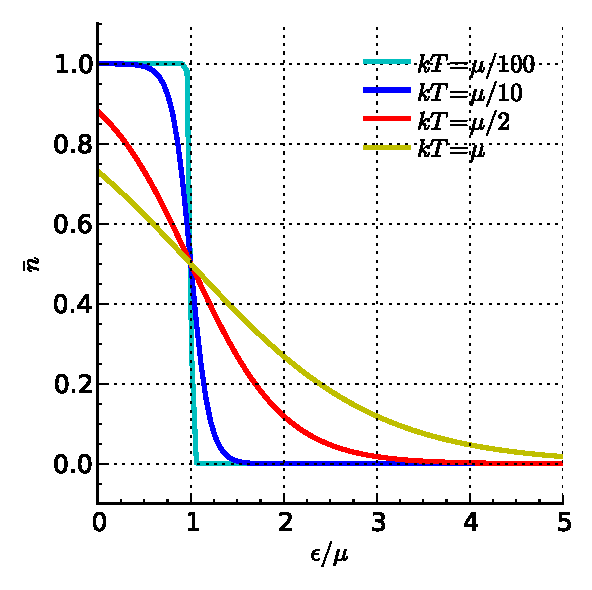
\includegraphics[scale=1]{fermidirac.pdf}
		 	\caption{Fermi-Dirac distribution [stolen; By Krishnavedala - Own work, CC BY-SA 3.0, \texttt{https://commons.wikimedia.org/w/index.php?curid=15478733}]\label{fermidirac}.}
		 \end{figure}
	 \item $\omega_{\beta,\mu}$ having finite density with infinite number of particles cannot be given by a vector or density matrix in $\mathcal{F}_a(L^2(\mathbb{R}^d))$. There is the famous Araki-Wyss representation associated to $\omega_{\beta,\mu}$, namely to $\varrho=\frac{ze^{-\beta H}}{\mathds{1}+ze^{-\beta H}}$. \begin{align}
	 H_{\varrho}=\mathcal{F}_a (\mathcal{H}) \otimes \mathcal{F}_a(\mathcal{H}) \qquad \Omega_{\varrho}=\Omega\otimes\Omega \\
	 \pi(a^*(\varphi))=b^*(\sqrt{1-\varrho}\varphi)\otimes \mathds{1}+(-\mathds{1})^{\mathcal{N}}\otimes b(\sqrt{\varrho}\varphi)\; .
	 \end{align}
	 If the density is a projection, i.e. $\varrho=\varrho^2$ (at $\beta=\infty$, see Eq. \eqref{eqn::limit_of_fermi_density}), then the two Fock-spaces have the interpretation: $\text{particles}\otimes\text{antiparticles}$. Check ($\mathcal{H}_\varrho,\Omega_{\varrho},T_{\varrho}$) is the GNS representation of $\omega_{\beta,\mu}$: \begin{align}
	 \langle \Omega_{\varrho},\pi_{\varrho}(a^*(\varphi)a(\varphi))\Omega_{\varrho}\rangle&=\langle \Omega\otimes \Omega,\left((-\mathds{1})^{\mathcal{N}}\otimes b(\sqrt{\varrho}\varphi)\right)\left((-\mathds{1})^{\mathcal{N}}\otimes b^*(\sqrt{\varrho}\psi)\right)\Omega\otimes \Omega)\\
	 &=\langle \Omega,b(\sqrt{\varrho}\varphi)b^*(\sqrt{\varrho}\psi)\Omega\rangle\\
	 &=\langle \sqrt{\varrho}\psi,\sqrt{\varrho}\varphi\rangle+\langle \Omega ,b^*(\sqrt{\varrho}\psi)b(\sqrt{\varrho}\varphi)\Omega\rangle\\
	 &=\langle \psi,\varrho\varphi\rangle=\omega_{\beta,\mu}(a^*(\varphi)a(\varphi))
	 \end{align}
	\end{itemize}
\end{remarks}
\section{Bosons}
Unlike in the fermionic case, the bosonic $b^{\#}(\varphi)$ are unbounded operators on Fock space and cannot represent a $C^*$-algebra. But $\Phi(\psi):=\frac{1}{\sqrt{2}}(b(\psi)+b^*(\psi))$ has a self-adjoint extension on $\mathcal{F}_s(\mathcal{H})$ and by Stone's theorem \begin{align}
W(t\psi):=\exp(it\Phi(\psi))\qquad (t\in\mathbb{R})\; ,
\end{align}
is a strongly continuous group of unitary operators. If $\mathcal{H}$ is a separable Hilbert space, the Weyl algebra $CCR(\mathcal{H})$ is the $C^*$-algebra generated by $\{W(\psi),\psi\in\mathcal{H}\}$ such that \begin{itemize}
	\item $W(\psi)=W(-\psi)^*$.
	\item $W(\varphi)W(\psi)=e^{-\frac{i}{2}\mathrm{Im}(\langle\varphi,\psi\rangle)}W(\varphi+\psi)$.
\end{itemize}
\begin{remarks}
	There are some remarks, mostly analogous to the Fermion case, to be made \begin{itemize}
		\item Again: $CCR(\mathcal{H})$ is unique up to $*$-isomorphisms.
		\item Here, if $h$ is a pre-Hilbert space, with $\overline{h}=\mathcal{H}$. Then $CCR(h)=CCR(\mathcal{H})$ iff $h=\mathcal{H}$.
		\item $W(0)=\mathds{1}$, $W(\psi)$ is unitary for all $\psi\in\mathcal{H}$.
		\item $\|W(\psi)-\mathds{1}\|=2$ for all $\psi\neq 0$ i.e. \underline{no} norm continuity in $\psi\mapsto W(\psi)$.
		\item The map $\psi\mapsto W(\psi)$ is called the \underline{Weyl quantization}.
	\end{itemize}
\end{remarks}
The finite volume thermal Gibbs state is again given by \begin{align}
\omega_{\beta,\mu}(A)=Z^{-1}_{\beta,\mu}\mathrm{Tr}_{\mathcal{F}_s(\mathcal{H})}(e^{-\beta K_{\mu}}A)\qquad Z_{\beta,\mu}=\mathrm{Tr}(e^{-\beta K_{\mu}}) \label{eqn::symm_gibbs}\; ,
\end{align}
where $K_{\mu}=\mathrm{d}\Gamma(H)-\mu\mathcal{N}$, on $CCR(\mathcal{H}_{\Lambda})$, $\Lambda\subset\mathbb{R}^d$, whenever $e^{-\beta K_{\mu}}\in I_1(\mathcal{F}_s(\mathcal{H}))$ (i.e. trace class).
\begin{lemma}
	$\exp(-\beta H)\in I_1(\mathcal{H})$ and $(H-\mu)>0$ (lower bound on the Hamiltonian) iff $\exp(-\beta K_{\mu})\in I_1(\mathcal{F}_s(\mathcal{H}))$.
\end{lemma}
\begin{remarks}
This basically means that for bosons the Gibbs state exists only for those chemical potentials $\mu\in\mathbb{R}$ such that $H-\mu>0$.
\end{remarks}
\begin{notes}
	$b^*(\varphi)b(\psi)$ is unbounded so $\mathrm{Tr}(e^{-\beta K_{\mu}}b^*(\varphi)b(\psi))$ is ''open to interpretation''.\\
	\underline{Formally} one would like to analyze the operator $\mathrm{Tr}\left( e^{-\frac{\beta K_{\mu}}{2}}b^*(\varphi)b(\psi)e^{-\frac{\beta K_{\mu}}{2}}\right)$, since one can prove that $b(\psi_1)\cdots b(\psi_n)e^{-\beta K_{\mu}}$ has a bounded, Hilbert-Schmidt closure which allows for the definition of \begin{align}
		\omega_{\beta,\mu}(b^*(\psi_1)\cdots b^*(\psi_n)&b(\varphi_m)\cdots b(\varphi_1))=\frac{1}{Z_{\mu,\beta}}\cdot \\ &\cdot \mathrm{Tr}\left(e^{-\frac{\beta K_{\mu}}{2}}b^*(\psi_1)\cdots b^*(\psi_n)b(\varphi_m)\cdots b(\varphi_1)e^{-\frac{\beta K_{\mu}}{2}}\right)\; ,
	\end{align}
	but one cannot use the cyclicity of the trace as we are dealing with unbounded operators (why that is, just imagine quantum mechanics with the momentum and space operator, if one could use cyclicity of the trace the commutator would be zero, while it really is unbounded). So to be a bit more precise: The bosonic $b(\varphi)b^*(\psi)$ are unbounded, so that it is a priori unclear if $\mathrm{Tr}(e^{-\beta K_{\mu}}b^*(\psi_1)\cdots b^*(\psi_n)b(\varphi_m)\cdots b(\varphi_1))$ is well-defined. In fact, it is not. However, it is \underline{formally} equal to \begin{align}\mathrm{Tr}\left(e^{-\frac{\beta K_{\mu}}{2}}b^*(\psi_1)\cdots b^*(\psi_n)b(\varphi_m)\cdots b(\varphi_1)e^{-\frac{\beta K_{\mu}}{2}}\right)\end{align}\; ,
\end{notes}
giving us the following lemma which will be proven in the exercises \begin{lemma}
Let $\Phi=(\varphi_1,\ldots,\varphi_m)$ and $B(\Phi):=b(\varphi_m)\cdots b(\varphi_1)e^{-\frac{\beta}{2}K_{\mu}}$. Then $B(\Phi)$ is closeable with bounded closure and $B(\Phi)\in I_2(\mathcal{F}(\mathcal{H}))$.\end{lemma}
IT follows that for $\Psi=(\psi_1,\ldots,\psi_n)$, $\Phi=(\varphi_1,\ldots,\varphi_m)$, $B(\Psi)^*B(\Phi)\in I_1(\mathcal{F}_s(\mathcal{H}))$ and we \underline{define}\begin{align}
\omega_{\beta,\mu}(b^*(\psi_1)\cdots b^*(\psi_n)b(\varphi_m)\cdots b(\varphi_1)):=\mathrm{Tr}(B(\Psi)^*B(\Phi))\;.
\end{align}
But this was just for details, for anything calculation related just use the above definition, combined with the relation\begin{align}
e^{-\frac{\beta K_{\mu}}{2}}b^*(\varphi)=b^*(e^{-\frac{\beta }{2}(H-\mu)}\varphi)e^{-\frac{\beta K_{\mu}}{2}}\; .\label{eqn::boson_relation}
\end{align} we can now formulate the proposition for the density distribution of the bosonic case
\begin{prop} Let $0<\beta<\infty$, $\mu\in\mathbb{R}$ and $H=H^{\dagger}$ such that $H-\mu>0$ and $e^{-\beta H}\in \mathcal{I_1(\mathcal{H})}$. Then \begin{align}
\omega_{\beta,\mu}(b^*(\varphi)b(\psi))&=\left\langle\psi, \frac{e^{-\beta(H-\mu)}}{1-e^{-\beta(H-\mu)}}\varphi\right\rangle\\
\omega_{\beta,\mu}(b^*(\varphi))&=0=\omega_{\beta,\mu}(b(\varphi))\; .
\end{align}
\end{prop}
\begin{notes}
	$1-e^{-\beta(H-\mu)}$ is invertible since $H-\mu>0$ implies $e^{-\beta(H-\mu)}<\mathds{1}$ and hence $\mathrm{Ker}(\mathds{1}-ze^{-\beta H})=\{0\}$.
\end{notes}
\begin{proof}
	The calculation is harder than in the Fermion case since we cannot use the cyclic properties of the trace. We have to commute our way to the goal \begin{align}
	\omega_{\beta,\mu}(b^*(\varphi)b(\psi))\overset{\eqref{eqn::boson_relation}}{=}&Z_{\beta,\mu}^{-1}\mathrm{Tr}\left(b^*(e^{-\frac{\beta}{2}(H-\mu)}\varphi)e^{-\beta K_{\mu}}b(e^{-\beta \frac{H-\mu}{2}}\psi)\right)\\
	=~~&\omega_{\beta,\mu}(b(e^{-\frac{\beta}{2}(H-\mu)}\varphi)b^*(e^{-\frac{\beta}{2}(H-\mu)}\psi))\mid \text{use CCR}\\
	=~~&\omega_{\beta,\mu}(b^*(e^{-\frac{\beta}{2}(H-\mu)}\varphi)b(e^{-\frac{\beta}{2}(H-\mu)}\psi))+\langle \psi, e^{-\beta (H-\mu)} \varphi\rangle\; .
	\end{align}
	Iterating this identity n-times gives \begin{align}
	\omega_{\beta,\mu}(b^*(\varphi)b(\psi))=&\omega_{\beta,\mu}\left(b^*(e^{-n\frac{\beta}{2}(H-\mu)}\varphi)b(e^{-n\frac{\beta}{2}(H-\mu)}\psi)\right)\\
	+&\sum_{j=1}^{n}\langle \psi, e^{-j\beta(H-\mu)}\varphi\rangle\; .
	\end{align}
	Since $H-\mu > C$ one has $\|e^{-n\frac{\beta}{2}(H-\mu)}\|\rightarrow 0$ as $n\rightarrow\infty$. For the second term we can use the Neumann series (i.e. the equivalent to the geometric series for operators) \begin{align}
	\sum_{j=1}^n\left(e^{-\beta(H-\mu)}\right)^j\rightarrow \left(\mathds{1}-e^{-\beta(H-\mu)}\right)^{-1}\left(e^{-\beta(H-\mu)}\right)\; .
	\end{align}
	The rest of the proposition follows as for fermions. 
	\end{proof}
	Technically (again) one would have to argue on the Weyl operators as they are the well-defined object. The analogous Lemma is \begin{align}
	\omega_{\beta,\mu}(W(\psi))=e^{-\frac{1}{4}\langle\psi, \frac{1+e^{-\beta(H-\mu)}}{1-e^{-\beta(H-\mu)}}\psi\rangle}\; .
	\end{align}
	Now the thermodynamic limit: If $H-\mu\geq C > 0$ uniformly in the volume, then the limit $L\rightarrow \infty$ can be taken as in the fermionic case. As a regular example take $\mathcal{H}_L=L^2\left(\left[-\frac{L}{2},\frac{L}{2}\right]^d\right)$, $H_L$ Dirichlet Laplacian with Eigenvalues $E_{\underline{n}}(L)=\frac{\pi^2}{L^2}(n_1^2+\cdots+n_d^2)$ whereby $\underline{n}\in \mathbb{N}^d$ and ground state energy \begin{align}
	E_{\underline{1}}(L)=\frac{\pi^2}{L^2}\rightarrow 0 \qquad (L\rightarrow \infty)\; .
	\end{align}
	Let $\mu<0$, so that $0<z=\exp(\beta \mu)<1$ and $H_L-\mu>-\mu>0$.
	\begin{theorem}
		$0<\beta<\infty$, $\mu<0$ and let $\omega_{\beta,\mu}^L$ be the Gibbs state over $CCR(\mathcal{H}_L)$, associated to $H_L$. Then \begin{align}
		\lim_{L\rightarrow\infty}\omega_{\beta,\mu}^L(A)=\omega_{\beta,\mu}(A)
		\end{align}
		for any $A\in CCR(\mathcal{H}_{L})$ and any $L$, where $\omega_{\beta,\mu}$ is the state on the $CCR(\mathcal{H})$ with two-point functions \begin{align}
		\omega_{\beta,\mu}(b^*(\varphi)b(\psi))=\frac{1}{(2\pi)^{d/2}}\int \overline{\hat{\psi}}(\xi)\frac{e^{-\beta(|\xi|^2-\mu)}}{1-e^{-\beta(|\xi|^2-\mu)}}\hat{\varphi}(\xi)\mathrm{d}\xi\; .
		\end{align}
	\end{theorem}
\begin{proof}
	Since the Weyl operators generate the whole algebra, it suffices to check the convergences on Weyl-operators $\omega_{\beta,\mu}^L(W(\psi))$. Bu the positive function \begin{align}
	x\mapsto \frac{1+e^{-\beta(x-\mu)}}{1-e^{-\beta(x-\mu)}}\qquad (x\geq \mu+C>\mu)
	\end{align}
	is bounded so that \begin{align}
	\langle \psi, \frac{1+e^{-\beta(H_L-\mu)}}{1-e^{-\beta(H_L-\mu)}}\psi\rangle
	\end{align}
	converges to the same expression with $H_L\leftrightarrow H$ namely \begin{align}
	\omega_{\beta,\mu}(W(\psi))=\exp\left(\frac{1}{(2\pi)^d}\int \overline{\hat{\psi}}(\xi)\frac{1+e^{-\beta(|\xi|^2-\mu)}}{1-e^{-\beta(|\xi|^2-\mu)}}\hat{\psi}(\xi)\mathrm{d}\xi\right)\; .
	\end{align}
\end{proof}
The finite volume density \begin{align}
\varrho_L(\beta,\mu)&=L^{-d}\sum_{\underline{n}}\omega_{\beta,\mu}^L(b^*(\psi_{\underline{n}})b(\psi_{\underline{n}}))\\
&=L^{-d}\sum_{\underline{n}}\frac{e^{-\beta(E_{\underline{n}(L)-\mu})}}{1-e^{-\beta(E_{\underline{n}}(L)-\mu)}}\; ,
\end{align}
is a monotone function of $\mu$, at fixed $\beta, L$, and since $\varrho_L(\beta,\mu)\rightarrow\infty$ as $\mu\rightarrow E_{\underline{1}}(L)$, its range is all $(0,\infty)$, so any density can be reached by choosing $\mu\in(-\infty,E_1(L))$. But this is not true if the TDL is taken first in $d\geq 3$ (which is of course the right order of limits). There the density is given by \begin{align}
\varrho(\beta, z)=\frac{1}{(2\pi)^{d/2}} \int \frac{e^{-\beta(|\xi|^2-\mu)}}{1-e^{-\beta(|\xi|^2-\mu)}}\mathrm{d}\xi \quad\text{ with }\quad Z=e^{\beta\mu}\;,
\end{align}
at $\mu=0$, the integrand scales like $|\xi|^{-2}$, which is integrable if $d\geq 3$. Natural question: How can a density 
\begin{align}
\overline{\varrho}>\varrho_C(\beta)=\varrho(\beta,1)=\frac{1}{(2\pi)^{d/2}}\int \frac{e^{- \beta |\xi|^2}}{1-e^{-\beta |\xi|^2}}\mathrm{d}\xi
\end{align} be obtained in the infinite volume limit? The short answer is that the excess density $\overline{\varrho}-\varrho_C(\beta)$ condensates into the ground state $\Rightarrow$ \underline{Bose-Einstein-condensation}.
First take periodic boundary conditions (for simplicity) and \begin{align}
z(L)=1-\frac{1}{(\varrho_0L^d)}\; .
\end{align}
Number of particles in the ground state \begin{align}
\mathcal{N}_{0,L}(\beta)&=\omega_{\beta,\mu}^L(b^*(\psi_0)b(\psi_0))\mid \text{use }E_0(L)=0\\&=\frac{z(L)}{1-z(L)}=\varrho_0 L^d-1\; ,\label{eqn::relation_nz}
\end{align}
so the density is constant. For non-ground states one finds ($\underline{n}\neq 0$) \begin{align}
\mathcal{N}_{\underline{n},L}(\beta)=(z(L)^{-1}e^{\beta E_{\underline{n}}(L)}-1)^{-1}\leq (\beta E_{\underline{n}}(L))^{-1}\leq \mathrm{const. }~L^2\; .
\end{align}
Hence: If $d=3$, the ground state $\psi_0$ is the only macroscopically occupied state (i.e. $\mathcal{N}_{0,L}(\beta)\sim L^3$). Precisely this means: Let $k=k(\underline{n})=\frac{4\pi^2}{L^2}(n_1^2+n_2^2+n_3^2)$. For any $\varphi\in C_c^{\infty}(\mathbb{R}^3)$ one then finds \begin{align}
L^{-3}\sum_{\underline{n}}\mathcal{N}_{k(\underline{n}),L}(\beta)\varphi(k(\underline{n}))\rightarrow \int \mathcal{N}_s(\beta,\xi)\varphi(\xi)\mathrm{d}\xi\; ,
\end{align}
where  \begin{align}\mathcal{N}_s(\beta,\xi)&=\overline{\mathcal{N}}(\beta,\xi)+\varrho_0 \delta(\xi) \\
\overline{\mathcal{N}}(\beta,\xi)&=(2\pi)^{-3}\frac{e^{-\beta|\xi|^2}}{1-e^{-\beta|\xi|^2}}\; .
\end{align}
Indeed, for any $\underline{n}\neq 0$: \begin{align}
\mathcal{N}_{\underline{n},L}(\beta)-(2\pi)^3\overline{\mathcal{N}}(\beta, k(\underline{n}))=(1-z^{-1}))e^{\beta E_{\underline{n}(L)}}\mathcal{N}_{\underline{k},L}(\beta)\overline{\mathcal{N}}(\beta,k(\underline{n}))(2\pi)^3
\end{align}
since $E_{\underline{n}}(L)=|k(\underline{n})|^2$. But $e^{\beta E_{\underline{n}}}\mathcal{N}_{k(\underline{n}),L}(\beta)\leq \mathrm{const.~}L^2$ so that \begin{align}
L^{-3}\sum_{\underline{n}\neq 0} \left|\mathcal{N}_{\underline{n},L}(\beta)-(2\pi)^3\overline{\overline{\mathcal{N}}}\right| \leq \frac{1}{\varrho_0 L^3}\mathrm{const.}L^3 \left(\left(\frac{2\pi}{L}\right)^3\sum_{\underline{n}\neq 0}\overline{\mathcal{N}}(\beta,k(\underline{n})\right)\;,
\end{align}
and the second factor is bounded above by $\int\overline{\mathcal{N}}(\beta,\xi)\mathrm{d}\xi$ which is finite in $d=3$, which conludes the argument. In terms of densities \begin{align}
\varrho_L(\beta,z(L))\rightarrow \varrho_0(\beta)=\varrho_C(\beta)+\varrho_0
\end{align}
Now this has been the easy discussion. Let us review some material and then tackle Bose-Einstein-condensation mathematically more rigorously. On the $CCR(\mathcal{H})$-algebra one has for the states \begin{align}
W(\psi)W(\varphi)=e^{\frac{i}{2}\mathrm{Im}\langle\psi,\varphi\rangle}W(\psi+\phi)\; ,\end{align}
which, on Fock spaces, translates to \begin{align}
W_{\mathcal{F}}(\psi)=e^{\frac{i}{\sqrt{2}}(b^{\dagger}(\psi)+b(\psi))}\;.
\end{align}
In finite volume one has $\exp^{-\beta H_L}\in I_1(\mathcal{H})$ and $H_{L}-\mu >0$ and \begin{align}
\omega_{\beta,\mu}^L(W(\psi))=\exp\left(\frac{1}{4}\left\langle \psi,\frac{\mathds{1}+e^{-\beta(H_L-\mu)}}{\mathds{1}-e^{-\beta(H_L-\mu)}}\psi\right\rangle\right)\; .
\end{align}
Now we want to take this into the TDL with $H_L=-\Delta_L$ with $H_L-\mu\geq C>0$ for all $L$ and obtain\begin{align}
\omega_{\beta,\mu}^L\overset{*}{\longrightarrow}\omega_{\beta,\mu} \text{ with } \omega_{\beta,\mu}(W(\psi))=\exp\left(\frac{1}{4}\left\langle \psi,\frac{\mathds{1}+e^{-\beta(H-\mu)}}{\mathds{1}-e^{-\beta(H-\mu)}}\psi\right\rangle\right)\; ,
\end{align}
where $(H\psi)(x)=(2\pi)^{-d/2}\int\hat{\psi}(\xi)|\xi|^2\mathrm{d}\xi$. For the density (in this case) one finds as a limit \begin{align}
\lim_{\mu\uparrow 0}\int\frac{e^{-\beta(|\xi|^2-\mu)}}{\mathds{1}-e^{-\beta(|\xi|^2-\mu)}}\mathrm{d}\xi = \int\frac{e^{-\beta|\xi|^2}}{\mathds{1}-e^{-\beta|\xi|^2}}\mathrm{d}\xi =: \varrho_{c}(\beta)\; ,
\end{align}
in finite volume the integral discretizes again and one obtains (with the counter for the multidimensional Eigenstate indices $\underline{n}$)\begin{align}
\varrho_{L}(\beta,Z)=\frac{1}{L^d}\sum_{\underline{n}}\frac{e^{-\beta(E_{\underline{n}}(L)-\mu)}}{\mathds{1}-e^{-\beta(E_{\underline{n}}(L)-\mu)}}\; ,
\end{align}
which diverges as $\mu$ goes towards the bottom of the spectrum. We confirm a second time that there is a difference in the order of limit taking. Let us look again at the periodic boundary conditions in the scaling limit, i.e. \begin{align}
Z(L)=1-\frac{1}{\varrho L^d}\; ,
\end{align}
using the previously found Eq. \eqref{eqn::relation_nz} we have \begin{align}
N_{\underline{0},L}(\beta)=\varrho_0L^d-1\; .
\end{align}
So the following inequality suggests itself \begin{align}
\mathcal{N}_{\underline{n},L}(\beta)\leq \mathrm{const.}~L^2\; .
\end{align}
Now: If $k(\underline{n})=\frac{4\pi^2}{L^2}(n_1^2+\ldots+n_d^2)$ and $E_{k(\underline{n})}(L)=|k(\underline{n})|^2$ \begin{align}
L^{-3}\sum_{\underline{n}}\mathcal{N}_{k(\underline{n}),L(\beta)}\varphi(k(\underline{n}))&\longrightarrow \int\mathcal{N}_s(\beta,\xi)\varphi(\xi)\mathrm{d}\xi\\
\mathcal{N}_s(\beta,\xi)&=\varrho_0\delta+\mathcal{N}(\beta,\xi)\\
&=\text{singular part} + (2\pi)^3\int\frac{e^{-\beta|\xi|^2}}{\mathds{1}-e^{-\beta|\xi|^2}}\;.
\end{align}
So by this way of taking the limit (as before), we see that the TDL part is recovered plus a singular part given by $\delta$. In terms of densities one has \begin{align}
\varrho_L(\beta,Z(L))\rightarrow\varrho_C(\beta)(2\pi)^{-3}+\varrho_C\; .
\end{align}
A more ''physical'' TDL would be gotten by fixing $\overline{\varrho}$ (here again with Dirichlet boundary conditions). Let $z_L$ be the solution of $\varrho(\beta,Z)=\overline{\varrho}$. If $\overline{\varrho}\leq \varrho_C(\beta)$. Let $\overline{Z}$ be the solution of $\varrho(\beta,Z)=\overline{Z}$. \begin{prop}
	Let $d\geq 3$. $0<\overline{\varrho}<\infty$, $0<\beta<\infty$: \begin{enumerate}
		\item If $\overline{\varrho}<\varrho_C(\beta)$, then $\lim_{L\rightarrow\infty}Z_L=\overline{Z}$.
		\item If $\overline{\varrho}>\varrho_C(\beta)$, then $\lim_{L\rightarrow\infty}Z_L=1$ (as in scaling limit) and \begin{align}
		L^{-d}\frac{Z_Le^{-\beta E_{\underline{1}}(L)}}{1-Z_Le^{-\beta E_{\underline{1}}(L)}}\; \longrightarrow \overline{\varrho}-\varrho_C(\beta)\qquad E_{\underline{1}}\text{ is GS in Dirichlet B.C}\; .
		\end{align}
	\end{enumerate}
\end{prop}
\begin{remarks}
	At fixed density, which is larger than the critical density, the activity must converge to $1$ as in the scaling limit discussed above, and the excess density $\overline{\varrho}-\varrho_C(\beta)$ goes into the ground state (i.e. exactly the statement we search).
\end{remarks}
\begin{proof}
	Note, that the exact convex analytics are not carried out here, so any convexity claim might be untrivial.\begin{enumerate}
	\item $\frac{az}{1-az}$ is convex for any $a>0$, so is $z\mapsto \varrho_L(\beta,z)$ and hence \begin{align}
	\frac{\partial \varrho_L}{\partial Z}(\beta, Z_2)\leq \frac{\varrho_{L}(\beta,Z_1)-\varrho_L(\beta,Z_2)}{Z_1-Z_2}\leq \frac{\partial \varrho}{\partial z}(\beta,z_1)\;,
	\end{align}
	for $z_2<z_1$. Moreover, \begin{align}\partial_z\frac{az}{1-az}=\frac{1}{z}\frac{az}{1-az}\frac{1}{1-az}\geq \frac{1}{z}\left(\frac{az}{1-az}\right)\; ,\end{align}

so that \begin{align}
\frac{\partial \varrho_L}{\partial Z}(\beta,Z_2)\geq \frac{1}{Z_L}\varrho_L(\beta,Z_L)\qquad [\text{use Dirichlet B.C.}]\; .
\end{align}
Also by Riemann approximation $\varrho(\beta,Z)\leq \varrho(\beta,Z)$ so that $Z_L\geq \overline{Z}$.  Combine these results with $Z_1=Z_L, Z_2=\overline{Z}$ to obtain \begin{align}
\frac{\varrho}{\overline{Z}}\leq \frac{\overline{\varrho}-\varrho_{L}(\beta,\overline{Z})}{Z_L-\overline{Z}}\; ,
\end{align}
namely \begin{align}
0\leq Z_L-\overline{Z}\leq \frac{\overline{Z}(\overline{\varrho}-\varrho_{L}(\beta,\overline{Z}))}{\varrho_L(\beta,\overline{Z})}\;.
\end{align}
\item Assume $Z_L\leq 1$. Then \begin{align}
\varrho_C(\beta)<\overline{\varrho}=\varrho_L(\beta,Z_L)\leq \varrho(\beta,Z_L)\leq \varrho(\beta,1)=\varrho_C(\beta)\; ,
\end{align}
which is a contradiction. Hence, $Z_L>1$ and $1<Z_L<e^{-\beta E_{\underline{1}}(L)}\rightarrow 1 \quad (L\rightarrow\infty)$.
\end{enumerate}
\end{proof}
\begin{theorem}
	Let $\mu_L$ be such that $z_L=e^{\beta\mu_L}$. Then (in $d\geq 3$) \begin{align}
	\omega_{\beta,\mu}^L\overset{*}{\longrightarrow}\omega_{\beta}\quad \text{ as }L\rightarrow\infty,\quad \text{ where}
	\end{align}\begin{enumerate}
		\item $\overline{\varrho}\leq \varrho_C(\beta)$, $\omega_{\beta}$ is given by \begin{align}\omega_{\beta}(W(\psi))=e^{-\frac{1}{4}\langle \psi, \frac{\mathds{1}+e^{-\beta (H-\overline{\mu})}}{\mathds{1}-e^{-\beta(H-\overline{\mu})}}\psi\rangle}\end{align} with $\overline{\mu}$ solving $\varrho(\beta,e^{\beta\mu})=\overline{\varrho}$.
		\item $\overline{\varrho}>\varrho_C(\beta)$, then $\omega_{\beta}(W(\psi))=\exp(-\frac{1}{4}q_{\beta}(\psi))$, where\begin{align}
		q_{\beta}(\psi)=2^{d+1}(\overline{\varrho}-\varrho_C(\beta))|\hat{\psi}(0)|^2+\int|\hat{\psi}(\xi)|^2\frac{1+e^{-\beta|\xi|^2}}{1-e^{-\beta|\xi|^2}}\mathrm{d}\xi\end{align}
	\end{enumerate}
\end{theorem}
\begin{remarks}
	\begin{enumerate}
		\item \begin{align}\varrho_C(\beta)=\int\frac{e^{-\beta|\xi|^2}}{1-e^{-\beta|\xi|^2}}\mathrm{d}\xi\end{align} which, with rescaling $\varrho=\beta^2\xi$, results in \begin{align}
		\varrho_C(\beta)=C\beta^{-d/2}\;,
		\end{align}
		so that, at fixed density, the BEC regime is obtained by lowering the temperature. BEC is a regime of high density/low temperature.
		\item Here, the thermal equilibrium state is not unique, but parametrised at fixed $\beta,\mu$ by the \underline{density}, $\frac{1}{\varrho}\in (\varrho_C(\beta),\infty)$. This is a way of looking at phase transitions.
		\item BEC for interacting particles is completely open.
	\end{enumerate}
\end{remarks}
GNS representatoin: $\omega_{\beta}$ at $\overline{\varrho}>\varrho_C(\beta):(\mathcal{H}_0,\pi_0,\varrho_0)$ \begin{align}
\mathcal{H}_0&=\mathcal{F}_s(\mathcal{H})\otimes \mathcal{F}_s(\mathcal{H})\otimes L^1(S^1)\\
\Omega_0&=\Omega\otimes\Omega\otimes\Omega\\
\pi_0(\omega(\psi))&=W_{\mathcal{F}}(\sqrt{1+\mu}\psi)\otimes W_{\mathcal{F}}(\sqrt{\mu}\psi)\otimes e^{i\alpha(\psi,\theta)}\\ \alpha(\psi,\theta)&=(2\pi)^{3/2}\sqrt{2\varrho_0} \left(\mathrm{Re}(\hat{\psi}(0))\cos\theta+\mathrm{Im}(\hat{\psi}(0))\sin\theta\right)\\
(\mu\psi)(x)&=\frac{1}{(2\pi)^3}\int\frac{e^{-\beta|\xi|^2}}{1-e^{-\beta|\xi|^2}\overline{\psi}(\xi)e^{i\xi x}}\mathrm{d}x \qquad \text{''Araki-woods''}\;.
\end{align}
 \section{KMS states}\label{sec::kms_states}
 We are now going to discuss the existence and uniqueness of equilibrium states in quantum statistical ensembles in a bit more detail. For the first part of this section we are going to set $\dim\mathcal{H}<\infty$, i.e. $\mathcal{H}=\mathbb{C}^n$, $\mathcal{A}=M_n(\mathbb{C})$. State: Given by $A\mapsto\mathrm{Tr}(\varrho A)$ with $0\leq \varrho\leq \varrho^*\leq \mathds{1}$ with $\mathrm{Tr}(\varrho)=1$. Dynamics are given by $\tau_t(A)=e^{itH}Ae^{-itH}$.\\
 {\centering\fbox{\parbox{0.8\linewidth}{\textbf{Gibbs variational principle:} Among all states, the equilibrium state(s) are minimizers of the free energy. }}\par}
 In the present case the free energy is given by \begin{align}
 \mathcal{F}_{\beta}:\mathcal{E}(\mathcal{A})&\longrightarrow \mathbb{R}\\
 \varrho &\longmapsto \mathcal{F}_{\beta}(\varrho)=E(\varrho)-\beta^{-1}S(\varrho)\;,
 \end{align}
 where $E(\varrho)=\mathrm{Tr}(\varrho H)$ is the energy and
 $S(\varrho)=-\mathrm{Tr}(\varrho\log\varrho)$ is the entropy.

\begin{prop}
	There exists exactly one minimizer of the free energy $\varrho_{\beta}=Z_{\beta}^{-1}e^{-\beta H}$ with $Z_{\beta}=\mathrm{Tr}(e^{-\beta H})$ and $F_{\beta}(\varrho_{\beta})=:f_{\beta}=-\beta^{-1}\log Z_{\beta}$.
\end{prop}
\begin{lemma}
	Let $0\leq A,B\leq \mathds{1}$, density matrices with $\ker B\subset \ker A$, then \begin{align}
	\mathrm{Tr}(A(\log A-\log B))\geq \frac{1}{2}\mathrm{Tr}(A-B)^2\; .
	\end{align}
\end{lemma}
\begin{proof}[Proof of lemma]
	Without loss of generality $\ker B=\{0\}$, and since we are in finite dimensions $B=\sum_i\beta_iP_i,\quad 0<\beta_i\leq 1$ and $A=\sum_j \alpha_jQ_j, \quad 0\leq \alpha_j\leq 1$. Now the function \begin{align}
	f(x):=\begin{cases}
	-x\log x\qquad  x&>0\\0 \qquad x&=0
	\end{cases}
	\end{align}
	is $C^0([0,\infty])\cap C^2([0,\infty])$, with $f''(x)=-\frac{1}{x}\quad (x>0)$ and thus f is concave. The Taylor-theorem now states that for $0\leq x<y\leq 1,~ \text{and }z\in (x,y)$
	\begin{align}
	f(y)-f(x)-(y-x)f'(y)=-\frac{1}{2}(x-y)^2f''(z)\geq \frac{1}{2}(x-y)^2\;\label{eqn::proof_of_ineq}
	\end{align}
	Hence we have the following relation \begin{align}
	\mathrm{Tr}(P_iQ_j(f(B)-f(A)+(A-B)f'(B)-\frac{1}{2}(A-B)^2\\=(f(\beta_i)-f(\alpha_j)+(\alpha_j-\beta_i)f'(\beta_i)-\frac{1}{2}(\alpha_j-\beta_i)^2)\mathrm{Tr}(P_iQ_j)\overset{\eqref{eqn::proof_of_ineq}}{\geq }0\; ,
	\end{align}
	which, when summing over i and j, gives \begin{align}
	0&\leq \mathrm{Tr}(-B\log B+A\log A +(A-B)(-\mathds{1}-\log B)-\frac{1}{2}(A-B)^2\\
	&=\mathrm{Tr}(A\log A-A\log B-\frac{1}{2}(A-B)^2)\;,
	\end{align}
	whereby $\mathrm{Tr}(A)=\mathrm{Tr}(B)=1$ was used. This proves the lemma.
\end{proof}
\begin{proof}[Proof of prop.]
	Use the lemma with $B=\varrho\beta$ and $A$ arbitrary and note that $\ker B=\{0\}$. One then has \begin{align}
	\beta(\mathcal{F}_{\beta}(A)f_{\beta})&=\beta \mathrm{Tr}(AH)+\mathrm{Tr}(A\log A)+\log Z_{\beta}\\
	&=\mathrm{Tr}(A\log A)-\mathrm{Tr}(A\log (Z_{\beta}^{-1}\exp(-\beta H)))\geq \frac{1}{2} \mathrm{Tr}((A-\varrho_{\beta})^2)\; .
	\end{align}

Since $(A-\varrho_{\beta})^2=(A-\varrho_{\beta})^*(A-\varrho_{\beta})\geq 0$, so that $\varrho_{\beta}$ is a minimizer of $\mathcal{F}_{\beta}$. Furthermore, $\mathrm{Tr}((A-\varrho_{\beta})^*(A-\varrho_{\beta}))=0$ implies $A=\varrho_{\beta}$, so that $\varrho_{\beta}$ is the unique minimizer.\end{proof}
Let $H$ be a matrix, so that $\tau_t(A)=e^{itH}Ae^{-itH}$ has an analytic extension $\tau_z(A)$ for all $z\in\mathbb{C}$. One has the following proposition \begin{prop}
	The Gibbs state is the unique state satisfying the $(\tau,\beta)-$KMS conditions \begin{align}
	\omega(A\tau_{i\beta}(B))=\omega(BA) \label{eqn::KMS_condition}\; .
	\end{align}
\end{prop}
\begin{proof}
	\begin{itemize}
		\item $\mathrm{Tr}(e^{-\beta H}Ae^{itH}Be^{-itH})\mid_{t=i\beta}=\mathrm{tr}(e^{-\beta H}BA)$ by cyclicity.
		\item Let $(\psi_i)_i$ be an eigenbasis of $H$, with eigenvalues $E_i$. Check the KMS-conditions \eqref{eqn::KMS_condition} for\begin{align}
		A=\langle \psi_j,\cdot\rangle\psi_i&=|\psi_i\rangle\langle\psi_j|\\
		B=\langle\psi_j,\cdot\rangle\psi_k&=|\psi_k\rangle\langle\psi| \; .
		\end{align}
		It results in \begin{align}
		lhs &= \mathrm{Tr}(\varrho|\psi_i\rangle\langle\psi_j|e^{-\beta E_k}\psi_k\rangle\langle\psi_l|e^{-\beta E_L})\\
		&= \langle \psi_l,\varrho\psi_i\rangle \delta_{jk}e^{-\beta(E_k-E_l)}\,.\\
		rhs&= \mathrm{Tr}(\varrho|\psi_k\rangle\langle\psi_l|\psi_i\rangle\langle\psi_j|)=\langle\psi_j,\varrho\psi_k\rangle\delta_{il}\;,
		\end{align}
		if Eq. \eqref{eqn::KMS_condition} holds, then $\varrho$ is diagonal in the eigenbasis with $\langle \psi_i,\varrho\psi_i\rangle = Ce^{-\beta E_i}$.
	\end{itemize}
\end{proof}
\begin{notes}The KMS condition relies only on the analiticity of $\tau_z(\beta)$ in a strip $S_{\beta}:=\{z\in \mathbb{C}:0<\mathrm{Im}(z)<\beta\}$ with continuous extension to $\overline{S}_{\beta}$.
	\end{notes}
\begin{definition}
	Let $(A,\tau)$ be a $C^*$-dynamical system, and $0<\beta,\infty$. A state $\omega$ on $\mathcal{A}$ is a $(\tau,\beta)$-KMS state if for any $A,B\in \mathcal{A}$ there exists a function $\mathcal{F}_{\beta}(A,B;t)$, which is analytic in $S_{\beta}$, continuous on $\overline{S}_{\beta}$ and satisfying the \textit{KMS boundary conditions} for $t\in\mathbb{R}$ \begin{align}
	\mathcal{F}_{\beta}(A,B;t)&=\omega(A\tau_t(B))\\
	\mathcal{F}_{\beta}(A,B;t+i\beta)&=\omega(\tau_t(B)A)\; .
	\end{align}
\end{definition}
\begin{remarks}
	For Gibbs one has $\mathcal{F}_{\beta}(A,B,z)=\mathrm{Tr}(\varrho_{\beta}A\tau_t(B))$, which satisfies the boundary condition.
\end{remarks}
\begin{notes}
	On $\mathcal{A}=\mathcal{M}_n(\mathbb{C})$, there is a unique $(\tau,\beta)-$KMS state. This is \textit{not true} in general, as illustrated by the Bose Gas in  the TDL. This non-uniqueness is a sign of phase-transition.
\end{notes}
An $A\in\mathcal{A}$ is called analytic for $\tau$ if $t\mapsto \tau_t(\mathcal{A})$ has an entire analytic extension $\tau_t(A)$.
\begin{theorem}
	A state $\omega$ on $\mathcal{A}$ is a $(\tau,\beta)$-KMS state, if and only if there is a dense $\tau$-invariant, $*$ subalgebra of analytic elements for $\tau$, call it $\mathcal{A}_{\tau}$, such that $\omega(A\tau_{i\beta}(B))=\omega(BA)$ for all $A,B\in \mathcal{A}_{\tau}$.
\end{theorem}
\begin{proof}
	$\Rightarrow$-direction: Let $A,B$ be analytic, i.e. $A,B\in\mathcal{A}_{\tau}$, then  $G(z)=\omega(A\tau_z(B))$ is analytic in $z$ and $G(t)=\omega(A\tau_t(B))=\mathcal{F}_{\beta}(A,B,t),t\in\mathbb{R}$, which follows by the KMS-boundary conditions. Hence $z\mapsto G(z)-\mathcal{F}_{\beta}(A,B;z)$ is analytic in $S_{\beta}$ (which is only the disk with positive imaginary part) and continuous in $\overline{S}_{\beta}$ and it vanishes on $\mathbb{R}$. By the Schwarz reflection-theorem it can be extended to an analytic function on $\{z\in\mathbb{C}:|\mathrm{Im}z|<\beta\}$, which still vanishes on $\mathbb{R}\subset \{z\in\mathbb{C}:|\mathrm{Im}~z|<\beta\}$. Hence, it vanishes everywhere and by continuity to $\{z\in\mathbb{C}||\mathrm{Im}z|\leq \beta\}$ it vanishes on the closed set as well. Hence \begin{align}
	G(i\beta)=\mathcal{F}_{\beta}(A,B,i\beta)=\omega(BA) \qquad \text{by KMS B.C.}\;,
	\end{align}
	which concludes, since $G(i\beta)=\omega(A\tau_{i\beta}(\beta))$.\\Now to the $\Leftarrow$-direction. Let $A,B\in\mathcal{A}_{\tau}$. We have that $\mathcal{F}(A,B,z):=\omega(A\tau_z(B))$ is analytic on $\mathbb{C}$ and \begin{align}
	\mathcal{F}(A,B;t)&=\omega(A\tau_t(B))\\
	\mathcal{F}(A,B;t+i\beta)&=\omega(A\tau_{i\beta}(\tau_t(B)))\overset{ass.}{=}\omega(\tau_t(B)A)\; ,
	\end{align}
which are the KMS boundary conditions. This extends to all $A,B\in\mathcal{A}$ by density and a bit of complex analysis.\end{proof}
We can now come to the first physical property, which serves as a first justification to see KMS states as the generalization of equilibrium states. \begin{prop}
	If $\omega$ is a $(\tau,\beta)$-KMS state. Then $\omega\circ \tau_t=0$is constant in time.. I.e. the equilibrium state is invariant under time evolution.
\end{prop}
\begin{proof}
	Let $A\in\mathcal{A}$ be analytic for $\tau$. Then $g(z):=\omega(\tau_z(A))$ is entire analytic and $g(z+i\beta)=\omega(\mathds{1}\tau_{i\beta}(\tau_z(A))=\omega(\tau_z(A)\mathds{1})=g(z)$. Hence: $g$ is periodic in the imaginary direction. Moreover \begin{align}
	|g(t+i\alpha)|&\leq \|\tau_{t+i\alpha}(A)\|=\|\tau_{i\alpha}(A)\| \\
	&\leq \sup\{\|\tau_{i\gamma}(A)\|:0\leq \gamma <\beta\} < \infty\; 
	\end{align}
	Hence, $g$ is entire analytic and bounded, and by the Liouville theorem $g$ is constant. This extends to all of $\mathcal{A}$ by density.
\end{proof}
\begin{notes}
As a technical side note: There is always a dense set of analytic elements.
\end{notes}
Now usually checking the KMS-conditions is a bit of a hassle but luckily there is an equivalent nice condition: \begin{theorem}[Energy-Entropy-Balance inquality (EEB)]
	A state $\omega$ over $\mathcal{A}$ is a $(\tau,\beta)-$KMS state iff\begin{align} -i\beta\omega(A^*\delta(A))\geq \omega(A^*A)\log \frac{\omega(A^*A)}{\omega(AA^*)}\end{align}
	for all $A\in D(\delta)$.
\end{theorem}
\begin{remarks}
	Usually one uses the following \begin{align}
	u\log\left(\frac{u}{v}\right)=\begin{cases}
	0&\colon u=0, v\geq 0\\
	+\infty &\colon u> 0, v=0\\
	u\log\left(\frac{u}{v}\right)&\colon else
	\end{cases}\; ,
	\end{align}
	which makes the function $(u,v)\mapsto u\log\left(\frac{u}{v}\right)$ a lower semicontinuous function.
\end{remarks}
\begin{remarks}
	If $\omega$ is a $\tau-$invariant state, namely $\omega\circ \tau_t=\omega$, then by the uniqueness of the GNS-representation there exists $H_{\omega}=H_{\omega}^*$ on $\mathcal{H}_{\omega}$ such that \begin{align}
		H_{\omega}\Omega_{\omega}&=0\\
		e^{itH_{\omega}}\pi_{\omega}(A)e^{-itH_{\omega}}&=\pi_{\omega}(\tau_t(A))\;,
		\end{align}
		and we say that $\exp(itH_{\omega})\cdot \exp(-itH_{\omega})$ is the unitary implementation of $\tau_t$ in $\mathcal{H}_{\omega}$ (s. exercises). 
\end{remarks}		
\begin{remarks}
	For $A\in\mathcal{A}$, we define two measures\begin{align}
	\mu_A(\Delta)&:=\langle\pi_{\omega}(A)\Omega_{\omega},P_{\omega}(\Delta)\pi_{\omega}(A)\Omega_{\omega}\rangle \sqrt{2\pi}\\
	\nu_A(\Delta)&:=\langle \pi_{\omega}(A^*)\Omega_{\omega},P_{\omega}(-\Delta)\pi_{\omega}(A^*)\Omega_{\omega}\rangle \sqrt{2\pi}	\; ,
	\end{align}
whereby $\Delta\subset\mathbb{R}$ is a Borel subset and $P_{\omega}$ is the projection valued measure of $H_{\omega}$, defined by \begin{align}
H_{\omega}=\int\lambda \mathrm{d}P_{\omega}(\lambda)\; .
\end{align}
Let $\tau_f(\Delta)=\int_{\mathbb{R}}f(t)\tau_t(\Delta)\mathrm{d}t$ for entire functions $f$ that is the the Fourier transform of a test function in $C_c^{\infty}(\mathbb{R})$. Then using that $P_{\omega}$ is projection valued, i.e. that it will drop down from the exponential row, since its exponent are all equal (second to third row)\begin{align}
\omega(A^*\tau_f(A))&=\int\langle \Omega_{\omega},\pi_{\omega}(A)^*\pi_{\omega}(\tau_t(A))\Omega_{\omega}\rangle f(t)\mathrm{d}t\\
&=\int f(t)\langle \pi_{\omega}(A)\Omega_{\omega},e^{itH_{\omega}}\pi_{\omega}(A)\Omega_{\omega}\rangle\mathrm{d}t\\
&=\int\int f(t)e^{it\lambda}\langle\pi_{\omega}(A)\Omega_{\omega},\mathrm{d}P_{\omega}(\lambda)\pi_{\omega}(A)\Omega_{\omega}\rangle\mathrm{d}t\\
&=\int \check{f}(\lambda)\mathrm{d}\mu_{A}(\lambda)\;,
\end{align}
whereby $\check{\cdot}$ indicates Fourier transform. Similarly one has \begin{align}
\omega(A\tau_f(A^*))&=\int \langle \pi_{\Omega}(A^*)\Omega_{\omega},\mathrm{d}P_{\omega}(\lambda)\pi_{\omega}(A^*)\Omega\rangle e^{-it\lambda}f(t)\mathrm{d}t\\
&=\int \langle \pi_{\omega}(A^*)\Omega_{\omega},\mathrm{d}P_{\omega}(\lambda) \pi_{\omega}(A^*)\Omega_{\omega}\rangle\check{f}(-\lambda)\\
&=\int \check{f}(\lambda)\mathrm{d}\nu_A(\lambda)\; .
\end{align}
Now $z\mapsto f(z)\tau_t(A)$ is an entire function, so that $\omega(A^*\tau_t(A))$ is as well and thus \begin{align}
\omega(A^*\tau_f(A))=\int f(\tau+i\beta)\omega(A^*\tau_{t+i\beta}(A))\mathrm{d}t\; .
\end{align}
If $\omega$ is a $(\tau,\beta)$-KMS state one finds furthermore \begin{align}
\omega(A^*\tau_f(A))=\int f(t+i\beta)\omega(\tau_t(A)A^*)\mathrm{d}t=\int\check{f}(\lambda)e^{t\beta \lambda}\mathrm{d}\nu_A\; .
\end{align}
And since this is true for any test function $\check{f}$ one obtains \begin{align}
\frac{\mathrm{d}\mu_{A}}{\mathrm{d}\nu_{A}}(\lambda)=e^{\beta\nu}\; .
\end{align}
In fact: this is again an if and only if condition. \end{remarks}
Now we can finally come to the proof of the theorem using all these relations: \begin{proof}
\begin{align}
\omega(A^*\delta(A))&=\langle\pi_{\omega}(A)\Omega_{\omega},\left[iH_{\omega},\pi_{\omega}(A)\right]\Omega_{\omega}\rangle\\
&=i\langle \pi_{\omega}(A)\Omega_{\omega},H_{\omega}\pi_{\omega}(A)\Omega_{\omega}\rangle\; ,
\end{align}
so that \begin{align}
\frac{-i\beta\omega(A^*\delta(A))}{\omega(A^*A)}=\frac{\beta \int \lambda \mathrm{d}\mu_A(\lambda)}{\int\mathrm{d}\mu_A(\lambda)}\; .
\end{align}
By Jensen's inequality one obtains \begin{align}
\exp\left(-\beta \frac{\int\lambda\mathrm{d}\mu_A(\lambda)}{\int\mathrm{d}\mu_A(\lambda)}\right)\leq \frac{\int e^{-\beta\lambda}\mathrm{d}\mu_A(\lambda)}{\int\mathrm{d}\mu_{A}(\lambda)}=\frac{\int\mathrm{d}\nu_A(\lambda)}{\int\mathrm{d}\mu_A}=\frac{\omega(AA^*)}{\omega(A^*A)}\; ,
\end{align}
taking the inverse relation gives \begin{align}
\exp\left(-i\beta\frac{\omega(A^*\delta(A))}{\omega(A^*A)}\right)\geq \frac{\omega(A^*A)}{\omega(AA^*)}\; ,
\end{align}
which, after taking a log, yields the $\Rightarrow$ direction. For the inverse direction we have \begin{align}
\omega(\tau_f(A)^*\tau_f(A))&=\int f(t)f(t')e^{i(t-t')\lambda}\langle \pi_{\omega}(A)\Omega_{\omega},\mathrm{d}P_{\omega}(\lambda)\pi_{\omega}(A)\Omega_{\omega}\rangle\mathrm{d}t\mathrm{d}t'\\
&=\int |\check{f}(\lambda)|^2\mathrm{d}\mu_A(\lambda)\; .
\end{align}
And analogously \begin{align}
\omega(\tau_f(A)\tau_f(A)^*)=\int|\check{f}(\lambda)|^2\mathrm{d}\nu_A(\lambda)\; .
\end{align}
And \begin{align}
-i\beta\omega(\tau_f(A)\delta(\tau_f(A)^*))=\int|\check{f}(\lambda)|^2(-\beta\lambda)\mathrm{d}\nu_A(\lambda)\; .
\end{align}
Now apply the EEB with $A^*\rightarrow \tau_f(A)$ and find that \begin{align}
\nu_A(\varphi\log\xi)\geq \nu_A(\varphi)\log \frac{\nu_A(\varphi)}{\mu_A(\varphi)}\; ,
\end{align}
where $\varphi(\lambda):=|\check{f}(\lambda)|^2$, $\xi(\lambda)=e^{-\beta\lambda}$ and similarly for $A\rightarrow \tau_f(A)$ \begin{align}
-\mu_A(\varphi\log\xi)\geq \mu_A(\varphi)\log \frac{\mu_A(\varphi)}{\nu_A(\varphi)}\;.
\end{align}
Since $\varphi$ is compactly supported, $\mathrm{supp}~\varphi\subset [m,M]$ one can thus write \begin{align}
-\beta M\varphi(\lambda)\leq \varphi(\lambda)\log\xi(\lambda)\leq -\beta m \varphi(\lambda) \quad \mid \quad \textbf{since }\log\xi(\lambda)=-\beta\lambda\;.
\end{align}
Hence we have that \begin{align}
-\beta m \nu_A(\varphi)&\geq \nu_A(\varphi)\log\frac{\nu_A(\varphi)}{\mu_A(\varphi)}\\
\beta M\mu_A(\varphi)&\geq \mu_A(\varphi)\log\frac{\mu_A(\varphi)}{\nu_A(\varphi)}\; .
\end{align}
And together this results in \begin{align}
\mu_A(\varphi)e^{-\beta M}\leq \nu_A(\varphi)\leq \mu_A(\varphi)e^{-\beta m}\; ,
\end{align}
namely \begin{align}
\frac{\mathrm{d}\mu_A(\lambda)}{\mathrm{d}\nu_A(\lambda)}=e^{\beta\lambda}\; ,
\end{align}
so that $\omega$ is a $(\tau,\beta)$-KMS state.
\end{proof}
\begin{prop}
Let $(\tau_t^{(n)})_{n\in\mathbb{N}}$ be a sequence of strongly continuous $1$-parameter groups of $*$-Automorphisms of $A$ such that for any $t$ and any $A\in\mathbb{A}$ one has \begin{align}
\|\tau_t^{(n)}(A)-\tau_t(A)\|\rightarrow 0 \qquad (n\rightarrow \infty)\; .
\end{align}
If $(\omega^{(n)})_{n\in\mathbb{N}}$ is a sequence of $(\tau^{(n)},\beta)$-KMS states, then any weak-$*$-accumulation point is a $(\tau,\beta)$-KMS state.
\end{prop}
\begin{proof}
Exercise. Some hints are to use the EEB, look at subsequences that converge independently take a limit and sandwich between inequalities. 
\end{proof}
This proposition is a general proof that, for example, the infinite volume limits of the free Bose/Fermi gases are KMS-states.\\
Now let us come to more characterisatins of equilibrium: \begin{itemize}
\item An equilibrium state is passive, i.e. in a cyclic process starting at equilibrium, no work can be extracted from the system on average.
\item An equilibrium state is stable, i.e. \begin{enumerate}
\item Structural stability: Equilibrium states depend continuously on the Hamiltonian.
\item Dynamical stability: A locally perturbed system returns to equilibrium if it was initially.
\end{enumerate}
\end{itemize}
\begin{example}
Let us assume for simplicity that $\dim \mathcal{H}<\infty$. Consider the setting of a time-dependent Hamiltonian $H(t)=H(t)^*, t\in[0,\tau]$ with $H(0)=H(\tau)$ and the initial state is a Gibbs state $\omega_{\beta}(A)=Z_{\beta}^{-1}\mathrm{Tr}(e^{-\beta H(0)}A)$. Let $U(t,t_0)$ be the solution of \begin{align}
i\frac{\mathrm{d}}{\mathrm{d}t}U(t,t_0)=H(t)U(t,t_0) \qquad \land \qquad U(t_0,t_0)=\mathds{1}\; ,
\end{align}
and let $U=U(T,0)$ be the driven evolution over one cycle $[0,T]$. work done by the system on the universe is given by \begin{align}
W=&\mathrm{Tr}(\varrho_{\beta}H(0))-\mathrm{Tr}(U\varrho_{\beta}U^*H(T))\\
=& \mathrm{Tr}(\varrho_{\beta}U^*[H,U]) \qquad \text{where }H=H(0)=H(T)\\
=& i\omega_{\beta}(U^*\delta(U))\; .
\end{align}
Given a $C^*$-dynamical system, a state is called passive if $-i\omega_{\beta}(U^*\delta(U))\geq 0$ for any $U\in\mathcal{A}$ unitary, $U\in D(\delta)$ and $U$ in the connected component of $\mathds{1}$.\end{example}
\begin{prop}
A $(\tau,\beta)$-KMS state is passive.
\end{prop}
\begin{proof}
Follows from the EEB-inequality \begin{align}
-i\beta\omega(A^*\delta(A))\geq \omega(A^*A)\log\frac{\omega(A^*A)}{\omega(AA^*)}\; ,
\end{align}
used with $A=U$.\end{proof}
\begin{remarks}
Now we shall prove in a general setting that passivity implies that no work is produced by a system in a cycle if the system starts at equilibrium. For that introduce the following on dynamics $\tau$ and a generator $\delta$. One says that \begin{align}
\delta_V=\delta + i[V,\cdot] \qquad V=V^*\in\mathcal{A}\; ,
\end{align}
is a local perturbation of $\delta$. Let $\tau_t^V=e^{t\delta_V}$. Now one has that \begin{align}
\frac{\mathrm{d}}{\mathrm{d}s}\tau_{-s}(\tau_s^V(A))=\tau_{-s}(i[V,\tau_s^V(A)])\; ,
\end{align}
so that \begin{align}
\left.\tau_t^V(A)-\tau_t(A)=\tau_{t-s}(\tau_s^V(A))\right|_{s=0}^{s=t}=\int_0^t\tau_{-s}(i[V,\tau_s^V(A)])\mathrm{d}s\; .
\end{align}
Iterating this identity gives \begin{align}
\tau_t^V(A)=\tau_t(A)+\sum_{k=1}^{\infty}\int_{{0\leq t_1\leq \ldots\leq t_k\leq t}} i[\tau_{t_1}(V),i[\tau_{t_2}(V),\ldots [\tau_{t_k}(V),\tau_t(A)]\cdots ]\mathrm{d}t_1\cdots \mathrm{d}t_k\; ,
\end{align}
which is norm convergent (recall that $\|[A,B]\|\leq 2\| A \| \| B\| $). In fact $\mathbb{C}\ni \lambda \mapsto \tau_t^{\lambda V}(A)\in\mathcal{A}$ is an entire function. The unitary function $\Gamma_V(t)$ solving \begin{align}
-i\frac{\mathrm{d}}{\mathrm{d}t}\Gamma_V(t)&=\Gamma_V(t)\tau_t(V)\\
\Gamma_V(0)&=\mathds{1}\;,
\end{align}
satisfies \begin{align}
\tau_t^V(A)\Gamma_V(t)=\Gamma_V(t)\tau_t(A)\; .
\end{align}
To illustrate that property think of $e^{it(H+V)}\cdot e^{-itH}$. We now define the work performed by the system along a cycle $V_t$, $t\in[0,T]$, with $V_0=V_t=0$, where the initial state is $\omega$, as \begin{align}
W:=-\int_0^T(\omega\circ \tau_t^{V_t})\left(\frac{\partial V_t}{\partial t}\right)\mathrm{d}t\; .
\end{align}
this can be justified, since the first factor is basically the time evolved to time $t$ and $\frac{\partial V_t}{\partial t}$ corresponds to the instantaneous change of energy. Note that \begin{align}
\frac{\mathrm{d}}{\mathrm{d}t}(\omega\circ \tau_t^V)(V_t)=\omega\circ \tau_t^V(\delta_{V_t}(V_t))+(\omega\circ \tau_t^V)\left(\frac{\mathrm{d}V_t}{\mathrm{d}t}\right)
\end{align}
and since \begin{align}
\delta_{V_t}(V_t)=\delta(V_t)+i[V_t,V_t]=\delta(V_t)\; ,
\end{align}
we have by integration of parts \begin{align}
W=\int_0^T(\omega\circ \tau_t^V)\underbrace{(\delta_{V_t}(V_t))}_{=\delta(V_t)}\mathrm{d}t-\underbrace{(\omega\circ\tau_t^V)(V_t)\mid_{t=0}^{t=T}}_{=0 (\text{since } V_0=V_T)}\;.
\end{align}
\end{remarks}
\begin{theorem}
Let $V_t\in C_c^1((0,\tau),\mathcal{A})$ and such that $D(\delta)\ni V_t$, $\delta\left(\frac{\partial V}{\partial t}\right)=\frac{\mathrm{d}\delta(V)}{\mathrm{d}t}$. If $\omega$ is a $(\tau,\beta)$-KMS state, then $W\leq 0$.\end{theorem} \begin{proof}
We claim that \begin{align}
W=i\omega(\Gamma_V(T)\delta(\Gamma_V(T)^*))\; ,
\end{align}
from the theorem follows by passivity of $\omega$. A calculation (write $\Gamma_V(T)=\Gamma$) gives \begin{align}
i\omega(\Gamma\delta(\Gamma^*))&=\int_0^T[\omega(i\dot{\Gamma}\delta(\Gamma^*)+\omega(\Gamma\delta(i\dot{\Gamma}^*))]\mathrm{d}t \qquad \mid \text{ use } -i\dot{\Gamma}=\Gamma\tau(V)\\
&=\int_0^T \omega(-\Gamma\tau(V)\delta(\Gamma^*)+\Gamma\delta(\tau(V)\Gamma^*))\\
&= \int_0^T\omega(\Gamma\underbrace{\delta(\tau(V))}_{=\tau(\delta(V))}\Gamma^*)\mathrm{d}t\\
&=\int_0^T\omega(\tau_t^V(\delta(V_t))\mathrm{d}t\quad \text{ since } \Gamma \text{ intertwines } \tau \text{ with } \tau^V\\
&=W\;.
\end{align}
\end{proof}
\begin{remarks}
Passivity implies Carnots version of the second law of thermodynamics. 
\begin{figure}
\centering
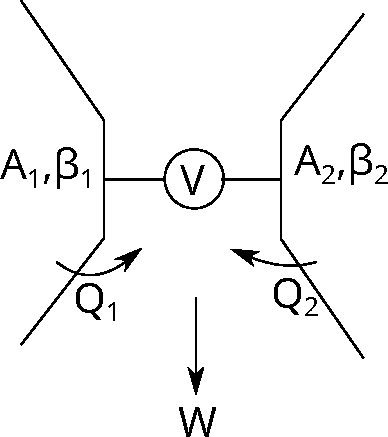
\includegraphics[scale=1]{carnot.pdf}
\caption{The system of the Carnot process, whereby one assumes without loss of generality that $\beta_1<\beta_2$.\label{fig::carnot}}
\end{figure}
Consider the system depicted in Fig. \ref{fig::carnot} with $\mathcal{A}=\mathcal{A}_1\otimes \mathcal{A}_2$, its free dynamics $\tau=\tau_1\otimes\tau_2$ with generator $\delta=\delta_1\otimes\mathds{1}+\mathds{1}\otimes\delta_2$. Call the initial state $\omega=\omega_{\beta_1}\otimes\omega_{\beta_2}$. This is a $(\sigma, \Lambda)$-KMS state, where\begin{align}
\sigma_t=\tau_{1,\beta_1t}\otimes \tau_{2,\beta_2t}\; ,
\end{align}
with generator $\gamma=\beta_1\delta_1\otimes\mathds{1}+\mathds{1}\otimes \beta_2\delta_2$. The Carnot machine is a cyclic local pertubation $V_t\in \mathcal{A}$. Total work perfomed by the system is then \begin{align}
W&=i\omega(\Gamma_V(T)\delta(\Gamma_V(T)^*))\\
&=i\omega(\Gamma(\delta_1\otimes\mathds{1})(\Gamma^*))+i\omega(\Gamma(\mathds{1}\otimes\delta_2)(\Gamma^*))\\
&=Q_1+Q_2\;.
\end{align}
Nwo $\beta_1 Q_1+\beta_2Q_2=i\omega(\Gamma\gamma(\Gamma^*))\leq 0$ by passivity. Hence: $\beta_1 Q_1+\beta_2(W.Q_q)\leq 0$, namely (with temperatures $T_1,T_2$\begin{align}
WT_1\leq -T_2Q_1+T_1Q_1 \overset{\text{hence}}{\longrightarrow} \frac{W}{Q_1}\leq \frac{T_1-T_2}{T_1}=1-\frac{T_2}{T_1}\; ,
\end{align}
i.e. the efficiency (work per heat) has an upper bound (the maximal efficiency) given by the temperature difference of both systems. We assumed that $Q_1>0$, i.e. that the machine pumps heat out of the system, to be able to produce work.
\end{remarks}
\begin{remarks}
Passivity is not sufficient to ensure that $\omega$ is a $(\tau,\beta)$-KMS state. One needs $\textit{complete passivity}$: For any $n\in\mathbb{N}$, the state $\bigotimes
_{i=1}^n\omega$ is passive for the $C^*$-dynamical system $(\bigotimes_{i=1}^n \mathcal{A},\bigotimes_{i=1}^n\tau)$.
\end{remarks}
By perturbation theory, KMS states are \textit{structurally stable} with respect to local perturbations, i..e if $\omega$ is a $(\tau,\beta)$-KMS state and $\delta_V=\delta+i[V,\cdot]$ is a local perturbation, then there is a $(\tau_V,\beta)$-KMS state $\omega_V$ such that $\|\omega-\omega_V\|\leq C\|V\|$. Moreover, the state $\omega_V$ can be represented as a density matrix in the GNS Hilbert space of $\omega$. In fact, there is a homomorphism between the set of $(\tau,\beta)$-KMS states, and the set of $(\tau_V,\beta)$-KMS states. 
The natural next questions that occur now are whether the structural map $\omega\mapsto\omega_V$ is realized dynamically, i.e. do we have $\omega\circ\tau_t^V\rightarrow\omega_V$ which would mark a return to equilibrium or thermalization. Reciprocally, does the convergence $\nu\circ \tau_t\rightarrow\omega(t\rightarrow\infty)$ impliy that $\omega$ is a $(\tau,\beta)$-KMS state?
For that consider the following system $(\mathcal{A},\tau)$, where we have a local perturbation \begin{align}
\tau_t(A)=e^{t\delta}(A) \qquad \delta_V(A)=\delta(A)+i[V,A]\; ,
\end{align}
whereby the latter relation generates dynamics $\tau^V(A)=e^{t\delta(V)}(A)$.
\begin{prop}
Let $V=V'\in\mathcal{A}$, and let $\omega^V$ be a $(\tau^V,\beta)$-KMS state and $\omega_+$ be a weak-$*$ accumulation point of \begin{align}
\omega^V\circ \tau_t\qquad (t\in\mathbb{R})\; .
\end{align}
If $\| [V,\tau_t^0(A)]\| \rightarrow 0$ as $t\rightarrow \infty$ and $VA\in\mathcal{A}$. Then $\omega_+$ is a $(\tau^0,\beta)$-KMS state.
\end{prop}
\begin{proof}
 Use the lower semi-continuity  of $u\log\frac{u}{v}$ to take the lower limit \begin{align}
 \omega_+(A^*A)\log\frac{\omega_t(A^*A)}{\omega_t(AA^*)}\leq& \lim\inf (\omega^V\circ \tau_t^0)(A^*A)\log\frac{(\omega^V\circ\tau_V^0)(A^*A)}{(\omega^V\circ\tau_t^0)(A^*A)}\\
 =& \liminf\limits_{t\rightarrow\infty} \omega^V(\tau_t^0(A)^*\tau_t^0(A))\log\frac{\omega^V(\tau_t^0(A)^*\tau_t^0(A))}{\omega^V(\tau_t^V(A)\tau_t^0(A^*)}\\
 \leq& \liminf\limits_{t\rightarrow\infty} -i\beta \omega^V(\underbrace{\tau_t^0(A)^*\delta_V(\tau_t^0(A))}_{=\delta(\tau_t^0(A)+i[V,\tau_t^0(A)]})\; .
 \end{align}
\begin{itemize}
\item First term converges to $-i\beta\omega_+(A^*\delta(A))$ since $\delta\circ\tau_t=\tau_t\circ \delta$
\item Second term converges to zero as \begin{align}
|\beta\omega^V(\tau_t^0(A)^*[V,\tau_t^0(A)])|\leq \beta \|A\| \|[V,\tau_t^0(A)]\| \rightarrow 0 \qquad (t\rightarrow \infty)
\end{align}
by assumption.
\end{itemize}
Hence $\omega_+(A^*A)\log\frac{\omega_+(A^*A)}{\omega_+(AA^*)}=-i\beta\omega_t(A^*\delta(A))$, i.e. $\omega_+$ solves the EEB inequality for the dynamics $\tau^0$ hence $\omega_+$ is a $(\tau^0,\beta)$-KMS state.
\end{proof}
The following is a more general theorem about KMS states, which will be stated without proof.
\begin{itemize}
\item ~[Assumption(A)]: For any $V=V^*$ in a dense subalgebra of $\mathcal{A}$ there exists $\lambda_V>0$ such that \begin{align}
\int_0^{\infty}\|[V,\tau_s^{\lambda\cdot V}(A)]\|\mathrm{d}s< \infty\;, 
\end{align}
for all $\lambda<\lambda_V$.
\item ~[Stability(S)]: For any V as above \begin{align}
\omega^{\lambda V}=\lim_{T\rightarrow\infty}\frac{1}{T}\int_0^T\omega_0\tau_t^{\lambda V}\mathrm{d}t
\end{align}
exists and $\|\omega-\omega^V\|\rightarrow 0$ as $\lambda\rightarrow 0$.
\end{itemize}
\begin{theorem}
Assume that $\omega$ is a factor state and that Assumption (A) holds. Then (S) holds iff $\omega$ is a $(\tau,\beta)$-KMS state.
\end{theorem}
\section{Symmetries}
\begin{definition}
A $*$-automorphism $\alpha$ of $\mathcal{A}$ is a symmetry of $(\mathcal{A},\tau)$ if \begin{align}
\alpha\circ\tau_t=\tau_t\circ \alpha \forall t \in \mathbb{R}\; .
\end{align}
\end{definition}
\begin{prop}
Let $\omega$ be a faithful $(\tau,\beta)$ KMS-state, i.e. $\omega(A^*A)>0$ for all $A\in\mathcal{A}$. Let $\alpha$ be a $*$-automorphism then \begin{enumerate}
\item $\omega\circ\alpha$ is a ($\alpha^{-1}\circ\tau\circ\alpha,\beta$)-KMS state.
\item If $\omega\circ \alpha = \omega$, then $\alpha$ is a symmetry of $(\mathcal{A},\tau)$.
\item If $\alpha$ is a symmetry, then $\omega\circ\alpha$ is a $(\tau,\beta)$-KMS state.
\end{enumerate}
\end{prop}
\begin{proof}
Prove these in parts: 
\begin{enumerate}
\item If $F$ is the analytic function associated to $\omega$ let $F_{\alpha}(A,B,z)=F(\alpha(A),\alpha(B),z)$ which is an entire function on $S_{\beta}$ and continuous in $\overline{S}_{\beta}$, and \begin{align}
F_{\alpha}(A,B; t)&=\omega(\alpha(A)\tau_t(\alpha(B)))\\
&=(\omega\circ \alpha)(A(\alpha^{-1}\circ\tau_t\circ\alpha)(B))\qquad (t\in\mathbb{R})\\
F_{\alpha}(A,B,t+i\beta)&=\omega(\tau_t(\alpha(B))\alpha(A))\\
&=(\omega\circ\alpha)((\alpha^{-1}\circ\tau_t\circ\alpha)(B)A)\; ,
\end{align}
so that $(\omega\circ\alpha)$ is an $((\alpha^{-1}\circ\tau\circ\alpha),\beta)$-KMS state.
\item A fundamental result of ''modular theory'' is the uniqueness of dynamics with respect to a state that is KMS. Now if $\omega\circ\alpha=\omega$, then $\omega$ is simultaneously a $(\tau,\beta)$-KMS state and a $((\alpha^{-1}\circ\tau\circ\alpha),\beta)$-KMS state (by the first part).
\item Follows from the first part and $\tau_t=\alpha^{-1}\circ\tau_t\circ\alpha$.
\end{enumerate}
\end{proof}
\begin{remarks}
In the case $\dim(\mathcal{H})<\infty$ a faithful state is given by a density matrix $\varrho>0$. Such a $\varrho$ determines a ''unique'' Hamiltonian $H$ such that $\varrho=\exp(-\beta H)$.
\end{remarks}
\begin{remarks}
The third part indicates that the set of $(\tau,\beta)$-KMS states is invariant under the action of a symmetry $\alpha$. If this is not the case for every single element in the set one speaks of symmetry breaking. There is a general criterion for the absence of symmetry breaking called the ''Mermin-Wagner theorem''.
\end{remarks}
For this theorem we will again first state the assumptions \begin{itemize}
\item~[Assumption(A)]: $\alpha$ is \textit{almost inner}, i.e. there exists $(U_n)_{n\in\mathbb{N}}$, $U_n\in \mathcal{A}^{\infty}$ unitary such that $U_n\in D(\delta)$ and \begin{align}
\lim\limits_{n\rightarrow\infty}\|\alpha(A)-U_n^*AU_n\| =0 \; .
\end{align}
\item~[Assumption(B)]: $\|\delta(U_m)\|\leq M$ for all $m\in\mathbb{N}$.
\end{itemize}
Typically $U_m$ are labelled by finite subsets $\Lambda_m$ of a lattice, in that case \begin{align}
\delta(U_m)\sim i[H_{\Lambda_m},U_m]\; ,
\end{align}
whose norm a priori goes like $|\partial\Lambda_m|$.
\begin{theorem}\label{thm::thm_with_assumptionsAB}
Let $\alpha$ be a symmetry of $(\mathcal{A},\tau)$. If (A) and (B) hold, then all $(\tau,\beta)$-KMS states are $\alpha-$invariant for all $0<\beta<\infty$.
\end{theorem}
\begin{proof}[Sketch of proof]
We will prove that there exists $C>0$, $C=C(\beta, M)$ such that \begin{align}
\omega(A^*A)\leq C(\omega\circ\alpha)(A^*A)\; ,
\end{align}
which implies that they are equal. The EEB for $U_mA$, $A\in\mathcal{A}$ \begin{align}
\omega(A^*A)\log\frac{\omega(AA^*)}{\omega(U_m A A^* U_m^*)}\leq -i\beta \underbrace{\omega(A^*U_m^*\delta(U_m A))}_{\mathclap{\omega(A^*U_m^*\delta(U_m)A)+\omega(A^*\delta(A))}}\; , \label{eqn::thm41proof}
\end{align}
on the left hand side we have \begin{align}
\log\frac{\omega(A^*A)}{\omega(U_mAA^*U_m^*)}=\underbrace{\log\frac{\omega(A^*A)}{\omega(AA^*)}}_{\text{ use } \frac{\mathrm{d}\mu_A}{\mathrm{d}v_A}=e^{\beta\lambda}}+\underbrace{\log \frac{\omega(AA^*)}{\omega(U_mAA^*U_m^*)}}_{\text{compares $\omega$ with $\omega\circ\alpha$}}
\end{align}
We now need upper bounds on the following two terms \begin{enumerate}
\item $-i\beta\omega(A^*U_m^*\delta(U_m)A)$.
\item $-i\beta\omega(A^*\delta(A))-\omega(A^*A)\log \frac{\omega(A^*A)}{\omega(AA^*)}$.
\end{enumerate}
for the first one use the assumption (B) to get \begin{align}
|\omega(A^*(U_m^*\delta(U_m))A)&\leq \| U_m\delta(U_m)\| \omega(A^*A)\\
&\leq M\omega(A^*A)\; .
\end{align}
For the second one note that $\omega(A^*\delta(A))=\langle\pi_{\omega}(A)\Omega_{\omega},H_{\omega}\pi_{\omega}(A)\Omega_{\omega}\rangle$ is unbounded. (Formally: Consider $A_n=P_nAP_n$, where $P_n=\int_{a_n}^{b_n}\mathrm{d}P(\lambda)$). So cover $\mathbb{R}$ by interval $[a_n,b_n]$, $|b_n-a_n|<1$ and $h_n^V\in C_c^{\infty}(\mathbb{R})$ with $\mathrm{supp}\check{h}_n\subset[a_n,b_n]$ and $\sum \check{h}_n^2=1$ and define \begin{align}
A_n=\tau_{h_n}(A)=\int h_n(t)\tau_t(A)\mathrm{d}t\in\mathcal{A}.
\end{align}
Then one finds that \begin{align}
-i\beta\omega(A_n^*\delta(A_n))=-i\beta\langle\pi(A_n)\Omega_{\omega},H_{\omega}\pi(A_n)\Omega_{\omega}\rangle=\ldots = \beta \int\lambda \check{h}_n(\lambda)^2\mathrm{d}\mu_A(\lambda)\;.
\end{align}
So one can approximate this as \begin{align}
|-i\beta\omega(A_n^*\delta(A_n))\leq \beta b_n\int\mathrm{d}\mu_A(\lambda)=\beta A_n \omega(A_n^*A_n)\;.
\end{align}
Furthermore one has \begin{align}
\omega(A_n^*A_n)=\int \check{h}_n(\lambda)^2\mathrm{d}\mu_A(\lambda)=\int \check{h}_n(\lambda)^2e^{\beta \lambda}\mathrm{d}\nu_A(\lambda)\geq e^{\beta a_n}\omega(A_nA_n^*)\; ,
\end{align}
so that \begin{align}
-\omega(A_n^*A_n)\log \frac{\omega(A_n^*A_n)}{\omega(A_nA_n^*)}\leq -\beta a_n\omega(A_n^*A_n)
\end{align}
Combine all these bounds in Eq. \eqref{eqn::thm41proof} to obtain \begin{align}
\omega(A^*_nA_n)\log \frac{\omega(A_nA_n^*}{\omega(U_mA_nA_n^*U_m^*}\leq -\beta \omega (A_n^*A_n)(M+\underbrace{(b_n-a_n)}_{<1})\; ,
\end{align}
Which bby taking the exponential yields \begin{align}
\omega(A_nA_n^*)\leq \omega(U_mA_nA_n^*U_m^*)e^{\beta(M+1)}
\end{align}
which is uniformly bounded with respect to $m$, so take $m\rightarrow\infty$ to obtain (with assumption (A)) \begin{align}
\omega(A_nA_n^*)&\leq (\omega\circ\alpha^{-1})(A_nA_n^*)e^{\beta(M+1)}\\
\omega(AA^*)&\leq C(\omega\circ\alpha^{-1})(AA^*)\;.
\end{align}
which implies that $\omega=\omega\circ \alpha^{-1}$ by an argument of convexity of the set of states, which will not be further elucidated here.
\end{proof}
There is actually another version of assumption (B) once could have made \begin{itemize}
\item~[Assumption(B')]: All $(\tau,\beta)$-KMS states are $\alpha^2$-invariant and \begin{align}
\|U_m^*\delta(U_m)+U_m\delta(U_m^*)\|< M\;.
\end{align}\end{itemize}
Whereby one can essentially repeat the previous proof with $(B')$ and repeat the estimate above with $U_m^*\leftrightarrow U_m$, and the sum of the two estimates becomes \begin{align}
\omega(A^*_nA_n)\log\frac{\omega(A_nA_n^*)^2}{\omega(U_mA_nA_n^+U_m^*)\omega(U_m^*A_nA_n^*U_m)}&\leq \beta\omega(A_n^*A_n)(M+w)\\
(\omega\circ\alpha^{-1})(A_nA_n^*)(\omega\circ\alpha)(A_nA_n^*)e^{\beta(M+1)}&\geq \omega(A_nA_n^*)^2\; ,
\end{align}
and if $\omega$ is KMS then $\omega\circ\alpha^{-1}$ is KMS, so by assumption \begin{align}
\omega\circ\alpha^{-1}=\omega\circ\alpha^{-1}\circ\alpha^2=\omega\circ\alpha\; .
\end{align}
Which ultimately leads to \begin{align}
\omega(A_nA_n^*)^2\leq (\omega\circ\alpha)(A_NA_N^*)^2E^{\beta(m+2)}
\end{align}
\chapter{On Phase transitions in quantum spin systems}
Let us first clear up what we mean with spin systems. We have a countable set $\Gamma$ with metric $d(\cdot,\cdot)$ (e.g. $\Gamma=\mathbb{Z}^{\nu}$). Then one writes the volume (e.g. the number of elements) of a subset $\Lambda\subset\Gamma$ as $|\Lambda|$ and defines the set $\mathcal{F}(\Gamma):=\{\Lambda\subset\Gamma\mid |\Lambda|<\infty\}$. For any $x\in\Gamma$, let $\mathcal{H}_x$ be finite dimensional (i.e. these are the spins): $\sup\dim\mathcal{H}_x<\infty$. For $\Lambda\in\mathcal{F}(\Gamma)^x$ one defines \begin{align}
\mathcal{H}_{\Lambda}=\bigotimes_{x\in\Lambda}\mathcal{H}_x\; .
\end{align}
We need to translate all our expressions into the language of these systems now
\begin{itemize}
\item Observables on $\Lambda\in\mathcal{F}(\Gamma)$ are defined on $\mathcal{A}_{\Lambda}\in\mathcal{L}(\mathcal{H}_{\Lambda})$ which are basically matrices. These are easily embedded into higher spaces $\Lambda_1\subset\Lambda_2$ as $\mathcal{A}_{\Lambda_1}\simeq \mathcal{A}_{\Lambda_1}\otimes\mathds{1}_{\mathcal{H}_{\Lambda_2\setminus \Lambda_1}}\subset \mathcal{A}_{\Lambda_2}$. Clearly for $A\in\mathcal{A}_X$, $B\in\mathcal{A}_Y$, $X\cap Y=\emptyset\Rightarrow[A,B]=0$, since \begin{align}
(A\otimes \mathds{1})\cdot(\mathds{1}\otimes B)=A\otimes B=(\mathds{1}\otimes B)(A\otimes\mathds{1})\; .
\end{align}
 Define the algebra of local observables as 
\begin{align} 
\mathcal{A}_{loc}=\bigcup_{\Lambda\in\mathcal{F}(A)}A_{\Lambda}\; .
\end{align}
and the complete algebra as $\mathcal{A}=\overline{\mathcal{A}_{loc}}^{\|\cdot\|}$, which is a $C^*$-algebra with an identity. \\
\item Any state $\omega$ on $\mathcal{A}$ is \textit{locally normal}, namely \begin{align}
\omega\mid_{\mathcal{A}_{\Lambda}}=\mathrm{Tr}(\varrho_{\Lambda}^{\omega}~\cdot~),\quad  \Lambda\in\mathcal{F}(\Gamma)\;,
\end{align}
i.e. one can think of $\omega$ on $\mathcal{A}_{loc}$ as the family of density matrices $\{\varrho_{\Lambda}^{\omega}:\Lambda\in\mathcal{F}(\Gamma)\}$.\\
\item Dynamics are given by maps\begin{align}
\Phi:\mathcal{F}(\Gamma)&\longrightarrow \mathcal{A}\\
X &\longmapsto \Phi(X)=\Phi(X)=\Phi(X)^*\in\mathcal{A}_X\; ,
\end{align}
which can be thought of as interactions between ''spins'' in the finite set $X\in\mathcal{F}(\Gamma)$. 
\item The Hamiltonian is given as the sum of local interactions\begin{align}
H_{\Lambda}=\sum_{x\subset\Lambda}\Phi(x),\quad \Lambda\in\mathcal{F}(\Gamma)\; .
\end{align}
\end{itemize}
A typical example of this is a two-body interaction $\Phi(X)=0$ if $|X|\neq 2$.\\
The finite volume dynamics \begin{align}
\tau_t^{\Lambda}(A)=e^{itH_{\Lambda}}Ae^{-itH_{\Lambda}}\; ,
\end{align}
has a well defined limit as $\Lambda\rightarrow\Gamma$, i.e. there exist $\tau$, a strongly continuous, 1-parameter group of automorphisms of $\mathcal{A}$, such that \begin{align}
\lim\limits_{\Lambda\rightarrow\Gamma}\|\tau_t^{\Lambda}(A)-\tau_t(A)\|\rightarrow 0\; , \quad \forall t\in\mathbb{R},A\in\mathcal{A}
\end{align}
under sufficient decay assumptions on $\|\phi(X)\|$ as diameter $\mathrm{diam}(X)$ (diameter being the spatial distance between the points as opposed to the dimension $|X|$) grows. And example is \begin{align}
\Phi(X)=0 \text{ whenever } \mathrm{diam}(X) > R, 
\end{align} i.e. basically finite-range interaction.\\
The \underline{Mermin-Wagner theorem} states the absence of continuous symmetry breaking in $\nu=1,2$. Here consider the same Hamiltonian on all sites $\mathcal{H}_x=\mathcal{H}$ for all $x\in\Gamma$. Furthermore, consider a continuous symmetry given by a compact connected Lie group $G$ (e.g. $SU(2)$). Assume there exists the following unitary representation of $G$ on $\mathcal{H}$ given by \begin{align}
U:G&\longrightarrow \mathcal{L}(\mathcal{H}) \\
g&\longmapsto U_g\; .
\end{align}
Whereby $U_gU_{g'}=U_{gg'}$, $U_{e}=\mathds{1}$ and $U_gU_g^*=U_g^*U_g=\mathds{1}$. Then this induces an action of $G$ on $\mathcal{A}_{\{x\}}$ given by $A\mapsto U_g^*A U_g$. Furthermore, on $\mathcal{A}_{\Lambda}, \Lambda\in\mathcal{F}(\Gamma)$ by $\otimes_{x\in\Lambda}U_g$ (whereby the implicit assumption that we take the same relation at every point is made) and yields $*$-automorphisms of $\mathcal{A}$ as the limit \begin{align}
\alpha_g(A)=\lim_{\Lambda\rightarrow\Gamma}\alpha_g^{\Lambda}(A) =\lim_{\Lambda\rightarrow\Gamma} \left(\bigotimes_{x\in\Lambda}U_g\right)^*A\left(\bigotimes_{x\in\Lambda}U_g\right)\; .
\end{align}
\begin{notes}
The limit exists for any $A\in\mathcal{A}_{loc}$ since $\alpha_g^{\Lambda}(A)$ is independent of $\Lambda$ for $\Lambda$ large enough, and it defines a bounded linear map of norm $1$. Hence the limit extends to the completion $\mathcal{A}$ of $\mathcal{A}_{loc}$.
\end{notes}
\begin{example}
$G=SU(2)$ with $U_g=\exp(2\pi i g S)$ where $S$ are the three spin matrices and $g$ is a point in the unit ball.
\end{example}
We will now prove the absence of symmetry breaking in $2D$-quantum spin systems. The $1D$-case is significantly easier and is left as an exercise.
\begin{theorem}
Let $\mathcal{A}$ be a quantum spin algebra with $\Gamma=\mathbb{Z}^2$, $\{\alpha_g:g\in G\}$ the action of a compact, connected Lie group $G$ on $\mathcal{A}$, and let $\phi$ be a $G-$invariant two-body interaction. $\alpha_g(\phi(x,y))=\phi(x,y)$ for all $(x,y)\in(\mathbb{Z}^2,\mathbb{Z}^2)$, $g\in G$. If \begin{align}
C:=\sup_{x\in\mathbb{Z}^2}\sum_{y\in\mathbb{Z}^2}\|\phi(x,y)\| d(x,y)^2<\infty,
\end{align}
then for any $0<\beta<\infty$, all $(\tau,\beta)$-KMS states are $G$-invariant, i.e. $\omega\circ\alpha_g=\omega$ $\forall g\in G$.
\end{theorem}
\begin{remarks}
We will use the notation $\Phi(X,Y)=\Phi({x,y})$ for a two-body interaction freely. Note that these are two two-dimensional objects, i.e. $x,y\in\mathbb{Z}^2$.
\end{remarks}
\begin{remarks}
This can be extended to n-body interactions.
\end{remarks}
\begin{remarks}
The condition for the constant, imposes sufficient decay on $\|\Phi(x,y)\|$ as $\mathrm{d}(x,y)\rightarrow\infty$. For a translation- and rotation-invariant interaction, the sharp decay condition is\begin{align}
\|\Phi(x,y)\|\leq C\mathrm{d}(x,y)^{-4}\; .
\end{align}
\end{remarks}
\begin{proof}
It suffices to check the conditions (A) and (B') of Theorem \ref{thm::thm_with_assumptionsAB}. It suffices to show the claim for an arbitrary one dimensional subgroup $H$ of $G$ \begin{align}
H=\mathbb{R}/\mathbb{Z}=S^1\; ,
\end{align} since if one considers rotations, one can always split them up into partial rotations around the coordinate axes. Let $S=S^*\in\mathcal{L}(\mathcal{H})$ be its generator such that\begin{align}
U_{\phi}=\exp(i\phi S),\quad \phi\in [0,2\pi)\; .
\end{align}
First define a smooth approximation of $\alpha_g$: Let $m\in\mathbb{N}$, $\Lambda_{m}=[-m,m]^2\cap\mathbb{Z}^2$, $\varphi_m:\mathbb{Z}^2\rightarrow[0,2\pi)$. One defines \begin{align}
\varphi_m(x)=\begin{cases}\phi & \colon x\in\Lambda_m \\
\phi(2-\mathrm{max}\{|x_1|,|x_2|\}/m)&\colon x=(x_1,x_2)\in\Lambda_{2m}\setminus\Lambda_m\\
0 & \colon x\in \mathbb{Z}^2\setminus\Lambda_{2m} \end{cases}\; ,\label{eqn::distance_dep_rotation}
\end{align}
and let \begin{align}
U_{\phi}(m)=\bigotimes_{x\in\Lambda_{2m}}\exp(i\varphi_m(x)S)\in\mathcal{A}_{\Lambda_{2m}}\subset\mathcal{D}(\delta)\; .\label{eqn::def_U_matrix}
\end{align}
Let $A\in\mathcal{A}_{loc}$ then there exists $m_0$ such that $A\in\mathcal{A}_{\Lambda_m}$ for all $m\geq m_0$. Then $U_{\phi}(m)^*AU_{\phi}(m)=\alpha_{\phi}(A)$ for all $m\geq m_0$. So that $U_{\phi}(m)^*\cdot U_{\phi}(m)\rightarrow\alpha_{\phi}(\cdot)$ on $\mathcal{A}_{loc}$. So by density of $\mathcal{A}_{loc}$ in $\mathcal{A}$ and boundedness of $\alpha_{\phi}\mid_{\mathcal{A}{loc}}$ the convergence extends to all of $\mathcal{A}$ and one recovers the assumption (A).\\
If $A\in\mathcal{A}_X$ for $X\in\mathcal{F}(\mathbb{Z}^2)$ then \begin{align}
\delta(A)=i[H,A]=i\sum_{\mathclap{\{x,y\}\cap X\neq \emptyset}}[\Phi(x,y),A]\; ,
\end{align}
so that 
\begin{align} 
U_{\phi}(m)^*\delta(U_{\phi}(m))&=i\sum_{\mathclap{\{x,y\}\in\mathbb{Z}^2\setminus \mathcal{N}_{m}}} (U_{\phi}^*(m)\Phi U_{\phi}(m))(x,y)\footnotemark-\Phi(x,y)\quad \text{with}\\\mathcal{N}_m &:=\{\{x,y\}: x,y\in\Lambda_m \text{ or } x,y\in\mathbb{Z}^2\setminus\Lambda_{2m}\} \;.
\end{align}
\footnotetext{It is not strictly necessary to put $(x,y)$ in front of the whole expression, as only the interaction term $\Phi$ depends on them. In this way it is easier to see though, that the angle by which $U$ rotates is influenced by the input argument as well, as can be seen from Eq. \eqref{eqn::def_U_matrix}, in which different angles are applied to different lattice sites (i.e. different elements of the tensor product). The input arguments kind of ''choose'' the relevant part of the tensor product.}
Since for all $\{x,y\}\in\mathcal{N}_m$ rotations happen around the same angle and the involved operators commute, i.e. \begin{align}
(U_m(\phi)^*\Phi U_m(\phi))(x,y)=\alpha_{\phi}(\Phi(x,y))=\Phi(x,y)\;.
\end{align}
For $\{x,y\}\in \mathbb{Z}^2\setminus\mathcal{N}_m$ one would rotate with different angles for the x and y part, thus giving a different interaction term compared to if one would not rotate. This is the definition of non-commuting operators.\\
With the action on $x$ defined as $S_x$ one can write \begin{align}
\varphi_m(x)S_x+\varphi_m(y)S_y&=\frac{\varphi_m(x)+\varphi_m(y)}{2}(S_x+S_y)+\frac{\varphi_m(x)-\varphi_m(y)}{2}(S_x-S_y)\\ &= E_m(x,y)+O_m(x,y)\; .
\end{align}
Note that $[E_m(x,y),O_m(x,y)]=0$ and $E_m(x,y)$ generates the same rotation at $x-$ and $y-$coordinates and thus\begin{align}\begin{split}
U_{\phi}(m)^*\Phi(x,y)U_{\phi}(m)=&\exp(i O_m(x,y))\exp(i E_m(x,y))\Phi(x,y)\\ &\cdot \exp(-iE_m(x,y))\exp(-i O_m(x,y))\end{split}\\
=& \exp(iO_m(x,y))\Phi(x,y)\exp(-i O_m(x,y))\; .
\end{align}
Because \begin{align}
\exp(i E_m(x,y))\Phi(x,y)\exp(-i E_m(x,y))=\alpha_{\frac{1}{2}(\varphi_m(x)+\varphi_m(y))}(\phi(x,y))=\Phi(x,y)\; .
\end{align}
Hence one can expand that expression to \begin{align}
U_{\phi}(m)^*\Phi(x,y)U_{\phi}(m) - \Phi(x,y)=\sum_{k=1}^{\infty} \frac{i^k}{k!}[O_m(x,y),[O_m(x,y),[\cdots[O_m(x,y),\Phi(x,y)]\cdots]\; . \label{eqn::merminproof}
\end{align}
Introducing the following notation \begin{align}
U_{\phi}(m)^*\delta(U_{\phi}(m))+U_{\phi}(m)\delta(U_{\phi}(m)^*)=i\sum_{x,y}\Delta_m(x,y)\; ,
\end{align}
and observe $U_{\phi}(m)\delta(U_{\phi}(m)^*)=U_{-\phi}(m)^*\delta(U_{-\phi}(m))$ and  that $O_m(x,y)$ is odd under $\phi\rightarrow -\phi$ so that all terms of odd order cancel out, yielding \begin{align}
\| \Delta_m(x,y)\| \leq 2 \sum_{k\geq 1} \frac{1}{(2k)!}\left(\frac{\varphi_m(x)-\varphi_m(y)}{2}\right)^{2k} \| \mathrm{ad}_{S_x-S_y}^{2k}(\Phi(x,y))\|\; ,
\end{align}
with \begin{align}
\| \mathrm{ad}_{S_x-S_y}^{2k}(\Phi(x,y))\| &\leq 2^{2k}(2\| S\| )^{2k}\|\Phi(x,y)\|\\
|\varphi_m(x)-\varphi_m(y)|^{2k}&\leq |\phi|^{2k}\left(\frac{d(x,y)}{m}\right)^2 \quad \text{since} \\|\varphi_m(x)-\varphi_m(y)|&\leq |\phi| \text{min}\left\{1,\frac{d(x,y)}{m}\right\}
\end{align}
Now one has $|\Lambda_m|=(2m+1)^2$ which cancels out the $1/m^2$ and in total obtains the bound on Eq. \eqref{eqn::merminproof} of \begin{align}
\sum_{\mathclap{x,y\in\mathbb{Z}^2\setminus\mathcal{N}_m}}\|\Delta_m(x,y)\| \leq \frac{4 e^{2\|S\||\phi|}}{m^2}\underbrace{\sum_{x\in\Lambda_m}\sum_{y\in\mathbb{Z}^2}}_{\mathclap{\leq (2m+1)^2\sup_{x\in\mathbb{Z}^2}\sum_{y\in\mathbb{Z}^2}}}\|\Phi(x,y)\| d(x,y)^2 \leq 36 C e^{2\|S\|\phi}\; ,
\end{align}
and thus we have a bound that is uniform in $m$, which gives us the bound needed for assumption (B'). We furthermore need symmtery invariance of the states under $\alpha^2$ to follow that they are $\alpha-$invariant as well. Since $\alpha_{\pi}^2=\mathrm{id}$ and $\omega\circ \alpha_{\pi}^2=\omega$ for all $(\tau,\beta)$-KMS states one thus finds by the theorem that $\omega\circ\alpha_{\pi}=\omega$ for all $(\tau,\beta)$-KMS states. Recursively $\omega\circ\alpha_{\pi/2n}=\omega \forall n,\omega$. But $\{\phi\in[0,2\pi):\phi=\sum_{n=0}^N a_n\left(\frac{\pi}{2n}\right)\mathrm{mod}~2\pi:a_n\in\mathbb{Z}, N\in\mathbb{N}\}=D$ is dense in $[0,2\pi)$. For any $A\in\mathcal{A}$: $\phi\mapsto\xi_A(\phi)=\omega(\alpha_{\phi}(A)-A)$ is continuous. Since $\xi_A|_D=0$, we conclude $\xi_A\equiv 0$ on $[0,2\pi)$.
\end{proof}
Now turning to higher dimensions similar general proofs have not been found yet and are the big open problems of statistical physics. What has been found for $\nu\geq 3$ is symmetry breaking for interacting systems in the antiferromagnetic Heisenberg-model (Dyson-Lieb-Simon, '78) \begin{align}
H_1 = \sum_{|x-y|=1}(S_x^1S_y^1+S_x^2S_y^2+S_x^3S_y^3)\; .
\end{align}
Whereby bounds of the following form are proven \begin{align}
\frac{1}{|\Lambda|}\sum_{x\in\Lambda}(-1)^{d(0,x)}\omega_{\beta,\Lambda}(S_0^3S_x^3)&\geq \kappa - \frac{1}{\beta }\sum_{\xi\in\Lambda^*}\frac{1}{E(\xi)}\overset{|\Lambda|\rightarrow\infty}{\longrightarrow}\frac{1}{\beta|\Lambda|}\sum\frac{1}{E(\xi)}\\&\rightarrow \frac{C}{\beta} \int_{[-\pi,\pi]}\frac{1}{E(\xi)}\mathrm{d}\xi\; ,
\end{align}
where $E(\xi)\sim |\xi|^2$ as $|\xi|\rightarrow 0$ if $\nu\geq 3$, the integral is convergent giving \begin{align}
\liminf \frac{1}{|\Lambda|}\sum(-1)^{|x|}\omega_{\beta,1}(S_0^3S_x^3)\geq \chi - \frac{\tilde{C}}{\beta}> 0\ ;, 
\end{align} 
if $\beta^{-1}$ is small enough. One finds long range order, i.e. \begin{align}\lim_{|x|\rightarrow\infty}\liminf_{|\Lambda|\rightarrow\infty} (-1)^{|x|}\omega_{\beta,\Lambda}(S_0^3S_x^3)>0\end{align}whenever $\nu\geq 3$ and $\beta^{-1}$ is small enough. This implies that the limiting states cannot be invariant under rotation. The key element of this proof really is the infrared bounds. Let $C_{\Lambda}(x)=(-1)^{|x|}\omega_{\beta,\Lambda}(S_0^3S_x^3)$ then the finiteness of the following was the clue to the proof \begin{align}
\frac{1}{|\Lambda|}\sum (-1)^{|x|}\omega_{\beta,\Lambda}(S_0^3S_x^3)=\hat{C}_1(0)=C_1(0)-\sum_{\xi\in\Lambda^*\setminus\{0\}}\hat{C}_{\Lambda}(\xi)\; ,
\end{align}
so one needs to control the amplitude of the small $\xi$ component of the correlation function. The ferromagnetic case though, is still completely open!
\backmatter
\end{document}